\addtocontents{toc}{\vspace{1em}}
\chapter{Correction}\label{chap:correction}
\chapintro{This chapter is based on results published in~\cite{Lohmann_2008_bpm}.}


\lettrine[findent=.2em,lines=2,nindent=0pt]{I}{n} the previous chapter, we focused on the verification of service compositions. Experimental results showed that it is possible to detect errors in service compositions with millions of states. In case an error was found, a counterexample is returned which shows how compatibility is violated.

Whereas errors can be \emph{detected} automatically (\ie, with tool support), the \emph{correction} of defective services is usually done manually. Correction steps include investigating the counterexample, determining which participant contains a design flaw, locating the error in the participant model, and finally fixing it. In addition, a subsequent verification is required to prove that the modification really corrected the service composition.

These correction steps are tedious, error-prone, and expensive, because they involve manual interference with the service composition. Hence, it would be desirable to automate the correction of incorrect service compositions to some extent. This is especially crucial, because fixing incorrect services is usually cheaper and takes less time than redesigning and implementing a correct service from scratch. In addition, information on how to adjust an existing service can help the designer \emph{understand} the error more easily compared to confronting him with an entirely newly synthesized service. We shall introduce a graph-based approach to calculate the minimal edit distance between a given defective service and synthesized correct services. This edit distance may help to automatically fix found errors while keeping as much of the service as possible untouched.

\medskip

In this chapter, we formalize, systematize, and to some extent automate the correction of service compositions. We thereby combine existing work on operating guidelines to characterize all strategies of a service (cf.~\autoref{chap:formal}) with similarity measures and edit distances known in the field of graph correction. We give a motivating example in \autoref{sect:corr:mot} and briefly sketch the correction approach in \autoref{sec:corr:concept}, before graph similarities are reviewed in \autoref{sect:graph}. In \autoref{sect:combine}, we define an edit distance which aims at finding the \emph{most similar} service from the set of all fitting services. To support the modeler, we further derive the required edit actions needed to correct the originally incorrect service. In \autoref{sect:experimental}, we present experimental results conducted with an implementation of the approach that serves as a proof of concept. \Autoref{sect:related} discusses related work. Finally, \autoref{sect:conclusion} is dedicated to a conclusion and gives directions for future research.





%%%%%%%%%%%%%%%%%%%%%%%%%%%%%%%%%%%%%%%%%%%%%%%%%%%%%%%%%%%%%%%%%%%%%%%%%%%%%%%
\section{Motivating example}
\label{sect:corr:mot}
%%%%%%%%%%%%%%%%%%%%%%%%%%%%%%%%%%%%%%%%%%%%%%%%%%%%%%%%%%%%%%%%%%%%%%%%%%%%%%%

%%%%%%%%%%%%%%%%%%%%%%%%%%%%%%%%%%%%%%%%%%%%%%%%%%%%%%%%%%%%%%%%%%%%%%%%%%%%%%
\begin{figure}%[t]
\centering
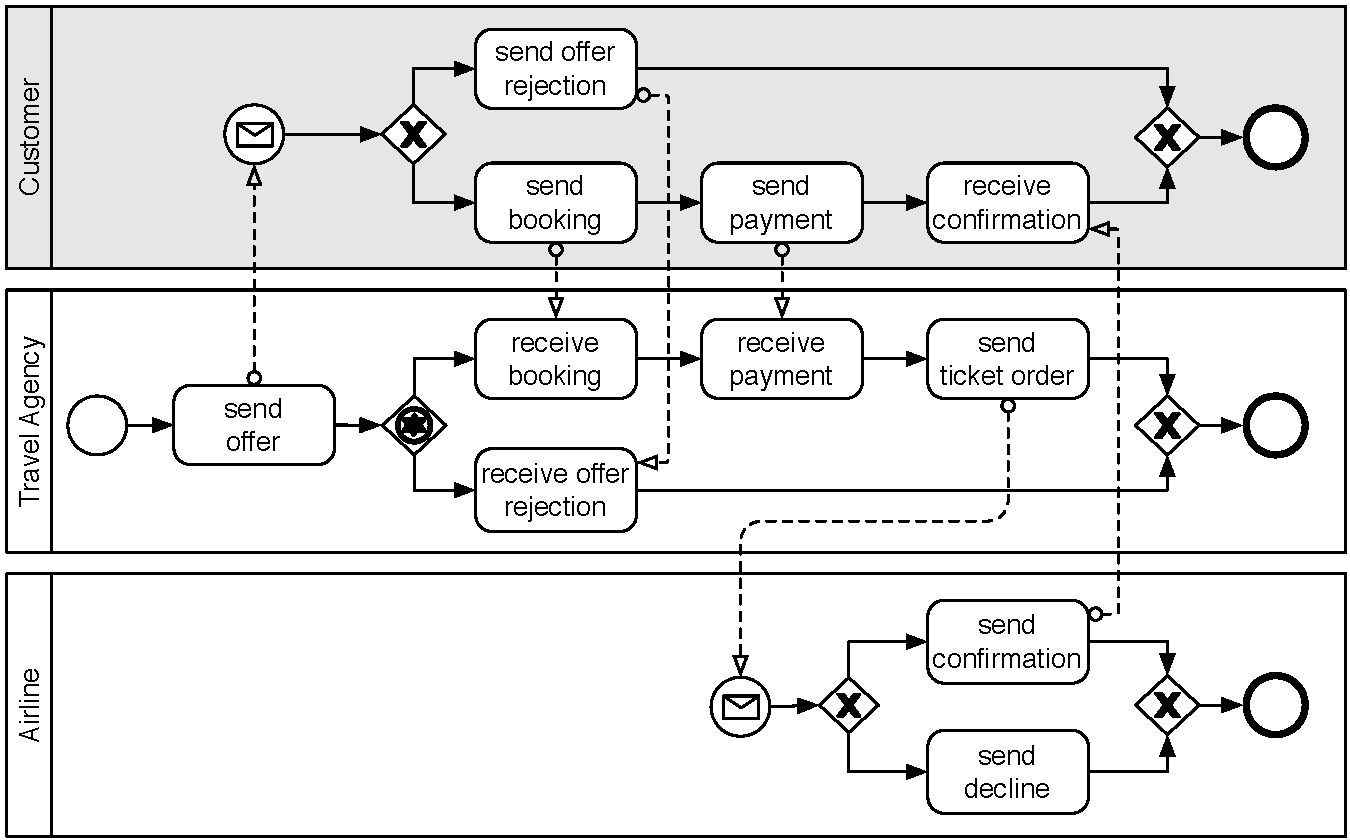
\includegraphics[scale=0.45]{correction/chor}
\caption{Incompatible choreography.}
\vspace{3em}
\label{fig:chor}
\subfigure[add branch to receive the decline message\label{fig:fix2}]{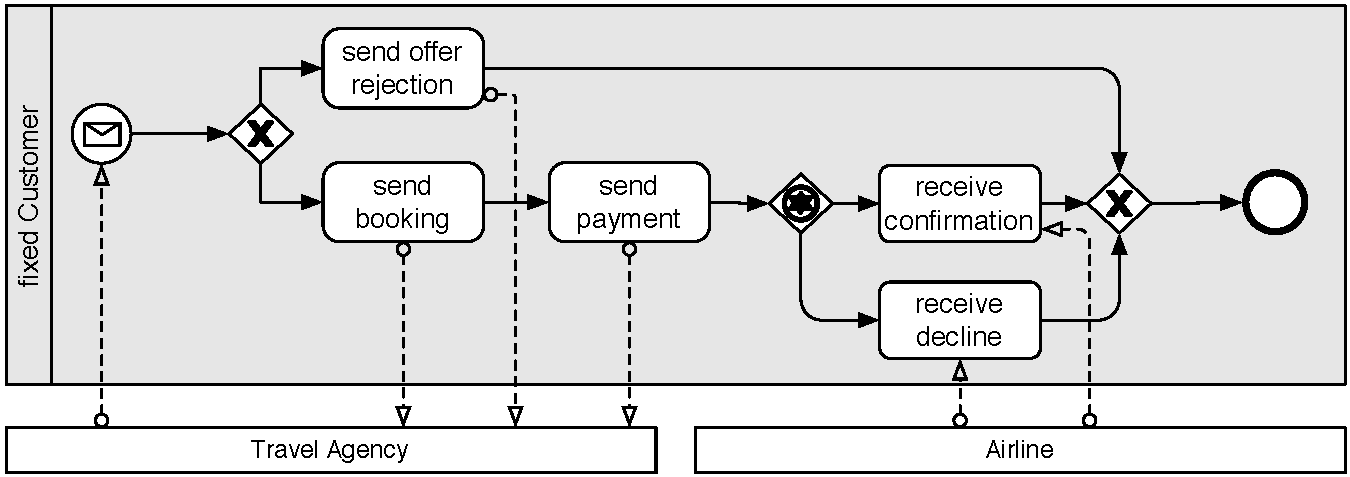
\includegraphics[scale=0.45]{correction/fix1}}\\
\subfigure[delete the booking branch\label{fig:fix1}]{\makebox[0.9\textwidth]{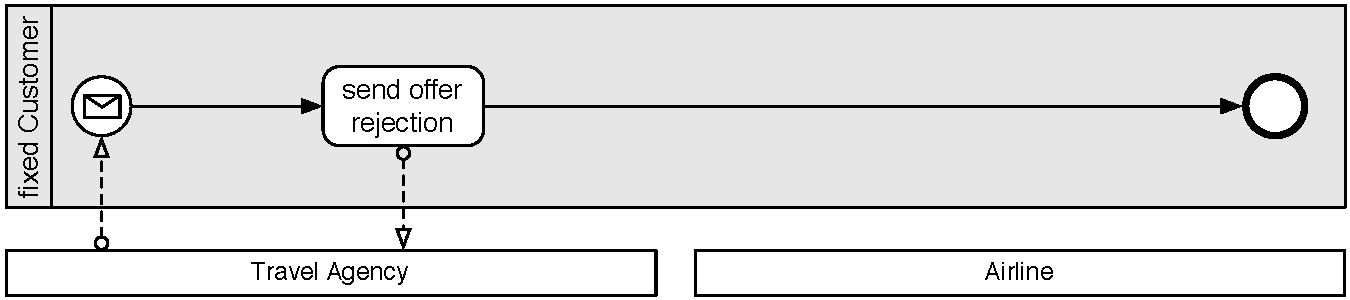
\includegraphics[scale=0.45]{correction/fix2}}}
\caption{Possible corrections of the customer service to achieve compatibility.}
\label{fig:fix}
\end{figure}
%%%%%%%%%%%%%%%%%%%%%%%%%%%%%%%%%%%%%%%%%%%%%%%%%%%%%%%%%%%%%%%%%%%%%%%%%%%%%%

As the running example for this chapter, consider an example choreography in \autoref{fig:chor}, which is similar to the example of the previous chapter and again visualized in \acronym{BPMN}~\cite{standard_bpmn}. It describes the interplay between a travel agency, a customer service, and an airline reservation system. The travel agency sends an offer to the client which either rejects it or books a trip. In the latter case, the travel agency orders a ticket at the airline service which either sends a confirmation or a decline message to the customer. The choreography contains a design flaw as the customer service does not receive the decline message. This leads to a deadlock in case the airline declines the ticket order, because the customer is not able to receive a decline message from the airline, but waits for a confirmation instead.

This incompatibility can be detected using state-of-the-art model checking tools which provide a trace to the deadlocking state, cf.~\autoref{chap:verification}. A concrete counterexample depends on the name of the states and transitions of the service automata modeling the choreography. At the level of detail of the depicted \acronym{BPMN} model, it could be
\begin{quote}
1.\ {send offer}, 2.\ {receive offer}, 3.\ {send booking}, 4.\ {send payment}, 5.\ {receive booking}, 6.\ {receive payment}, 7.\ {send ticket order}, 8.\ {receive ticket order}, 9.\ {send decline}.
\end{quote}
This trace, however, gives no insight \emph{which service} has to be changed in \emph{which manner} to avoid the deadlock. Thus, an iteration of manual corrections followed by further checks is necessary to finally remove the deadlock. Even though it is obvious how to correct the flawed example, the manual correction of choreographies of a larger number of more complex services is complex and error-prone, if not impossible.

Moreover, even for this simple choreography there exists a variety of possibilities to correct the customer's service. \Autoref{fig:fix} depicts two possible corrections to achieve compatibility. Although either service would guarantee compatibility, the service in \autoref{fig:fix2} is to be preferred over the one in \autoref{fig:fix1} as it is ``more similar'' to the original service. Albeit this preference is psychological and is unlikely to be rigorously formalizable, the usage of similarities is accepted in the area of error explanation~\cite{GroceCKS_2006_sttt}. The tool chain presented in the previous chapter synthesizes a participant service independently of an existing incorrect service which is either most-permissive (cf.~\autoref{def:synthesis}) or reduced (cf.~\autoref{def:synthesisreduced} and~\cite{Weinberg_2008_wsfm}). Whereas the former most-permissive strategy is usually much larger than a manually specified service, the latter result may be a correct, yet unintuitive result such as the service in \autoref{fig:fix1}. Hence, the remainder of this chapter is dedicated to the synthesis of a service which not only ensures compatibility of the overall composition, but also is as close to the (incorrect) original service as possible.





%%%%%%%%%%%%%%%%%%%%%%%%%%%%%%%%%%%%%%%%%%%%%%%%%%%%%%%%%%%%%%%%%%%%%%%%%%%%%%%
\section{Correcting incompatible choreographies}\label{sec:corr:concept}
%%%%%%%%%%%%%%%%%%%%%%%%%%%%%%%%%%%%%%%%%%%%%%%%%%%%%%%%%%%%%%%%%%%%%%%%%%%%%%%

In the remainder of this chapter, we show how the correction procedure of an incompatible service choreography can be supported by automatically providing recommendations for the modeler. This procedure includes the calculation of the candidates for the correction on the one hand and the choice which candidate to take can be automated on the other hand. To provide some intuition, we show how the choreography \emph{completion} described in \autoref{chap:verification} can also used to \emph{correct} choreographies.

Consider an incompatible choreography of $n$ participants, $A_{1}\oplus\cdots\oplus A_{n}$. As mentioned before, a counterexample (\eg, a deadlock trace) usually does not give enough information \emph{how} to fix \emph{which} service to achieve compatibility. To find a candidate service which can be changed such that the entire choreography is compatible, we propose the following steps:

\begin{niceenumerate}
\item We check for each service the necessary correctness criterion: If a service taken for itself is not controllable, then there exists no environment in which this service runs correctly\,---\,in particular not the choreography under consideration. In that case, that service has to be radically overworked toward controllability using the diagnosis algorithm of \autoref{chap:diagnosis}.

\item We remove one participant, say $A_{i}$. The resulting choreography $\mathit{Chor_{i}}:=A_{1}\oplus\cdots\oplus A_{i-1}\oplus A_{i+1}\oplus\cdots\oplus A_{n}$ can be considered as one large service with an interface to $A_i$. If this large service is controllable, then there exists a service $A_{i}'$ which interacts in a compatible manner with the other participants of the choreography; that is, $\mathit{Chor_{i}}\oplus A_{i}'$ is compatible. In \autoref{chap:verification}, we presented a complete tool chain for this participant synthesis for \acronym{WS-BPEL}-based choreographies. We shall discuss the case in which $\mathit{Chor_{i}}$ is uncontrollable later.
\end{niceenumerate}

As motivated in the introduction, the mere replacement of $A_{i}$ by $A_{i}'$ is not desirable, because $A_{i}'$ is synthesized independently of the faulty service $A_i$ and totally ignores its structure. Hence, it may be very different to the original, yet incorrect service $A_{i}$. Instead of synthesizing \emph{any} fitting service (such as the service in \autoref{fig:fix1}), we are interested in a corrected service which is most similar to $A_{i}$. To this end, we can use the operating guideline of $\mathit{Chor_{i}}$, because it characterizes the set of \emph{all} fitting partners. \Autoref{fig:space} illustrates this.

It is important to stress that any automated method can only provide \emph{suggestions} to change a model, and these suggestions always need to be evaluated manually. To this end, the suggestions should be as local as possible.

%%%%%%%%%%%%%%%%%%%%%%%%%%%%%%%%%%%%%%%%%%%%%%%%%%%%%%%%%%%%%%%%%%%%%%%%%%%%%%
\begin{figure}[t]
\centering
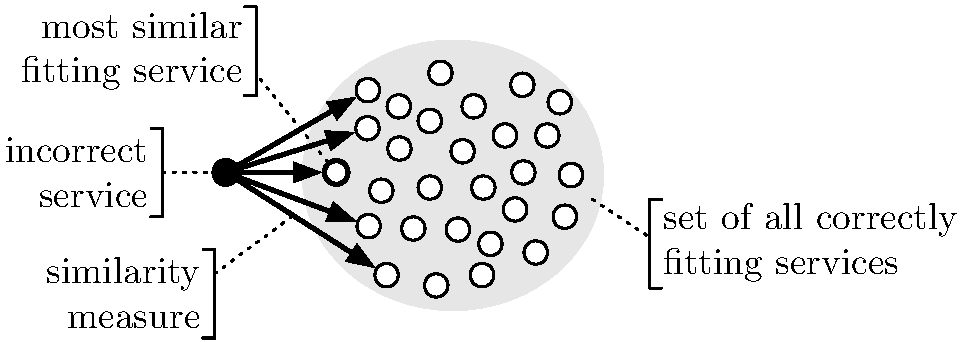
\includegraphics[scale=0.45]{correction/space}
\caption{The operating guideline as characterization of all correct services can be used to find the most similar correct service.}
\label{fig:space}
\end{figure}
%%%%%%%%%%%%%%%%%%%%%%%%%%%%%%%%%%%%%%%%%%%%%%%%%%%%%%%%%%%%%%%%%%%%%%%%%%%%%%

%%%%%%%%%%%%%%%%%%%%%%%%%%%%%%%%%%%%%%%%%%%%%%%%%%%%%%%%%%%%%%%%%%%%%%%%%%%%%%
\begin{figure}[t]
\centering
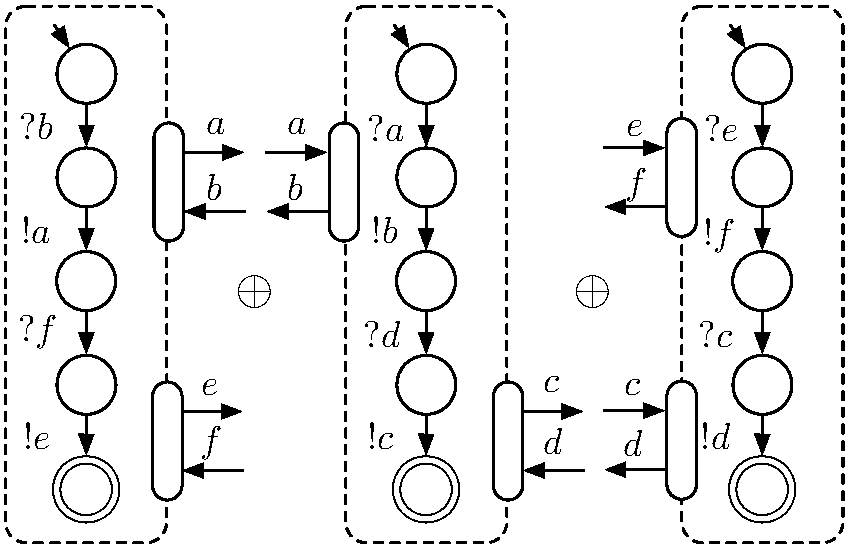
\includegraphics[scale=0.45]{correction/counter}
\caption{An incompatible composition of controllable services.}
\label{fig:corr:counter}
\end{figure}
%%%%%%%%%%%%%%%%%%%%%%%%%%%%%%%%%%%%%%%%%%%%%%%%%%%%%%%%%%%%%%%%%%%%%%%%%%%%%%

The problem statement of this chapter is as follows: Given an incompatible service composition $A_1\oplus\cdots\oplus A_n$ (\eg, the choreography in \autoref{fig:chor}) and a fault service $A_{i}$ (\ie, a ``scapegoat'' such as the customer service in \autoref{fig:chor}) such that $\mathit{Chor_{i}}$ is controllable, what are minimal edit actions to change $A_{i}$ to $A_{i}^{*}$ such that $A_{1}\oplus\cdots\oplus A_{i-1}\oplus A_{i}^{*}\oplus A_{i+1}\oplus\cdots\oplus A_{n}$ is compatible?

Unfortunately, controllability of each participating services $A_1,\ldots,A_n$ does not guarantee controllability of $\mathit{Chor_{i}}$. \Autoref{fig:corr:counter} shows an incompatible composition of three controllable services in which the removal of any single service yields an uncontrollable service. This is because of a cyclic dependency between any pair of participants. As any pair of remaining services is uncontrollable, no suggestion can be derived from the composition which service needs to be repaired. In such a situation, we need to diagnose the reasons which lead to uncontrollability of $\mathit{Chor_{i}}$, choose a different service to repair, or remove a second service. In the remainder of this chapter, \emph{we assume that we can identify a single service for correction}.


\paragraph{Example.}

\Autoref{fig:corrog} depicts an operating guideline of the composition of the travel agency and the airline. The service automaton of \autoref{fig:corsa} is structurally matched by the operating guideline and satisfies all but one formula: It does not satisfy the formula $\varphi(q_2)={?c}\wedge{?d}$ of the operating guidelines's state $q_2$, because the service automaton does not receive a decline message ($d$) in the matched state $q_1$.

%%%%%%%%%%%%%%%%%%%%%%%%%%%%%%%%%%%%%%%%%%%%%%%%%%%%%%%%%%%%%%%%%%%%%%%%%%%%%%
\begin{figure}
\centering
\subfigure[$A_\textit{cust}$\label{fig:corsa}]{\makebox[0.2\textwidth]{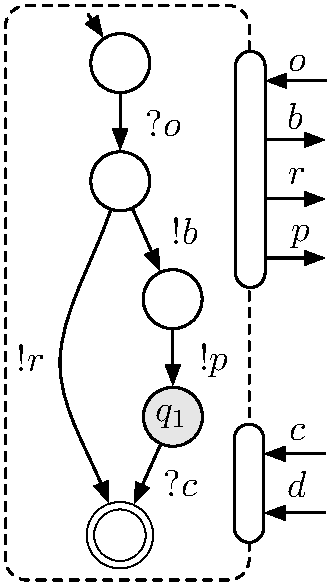
\includegraphics[scale=0.45]{correction/sa}}}\hspace{6em}%\hfill
\subfigure[$OG_{A_\text{agency}\oplus A_\text{airline}}^1$\label{fig:corrog}]{\makebox[0.4\textwidth]{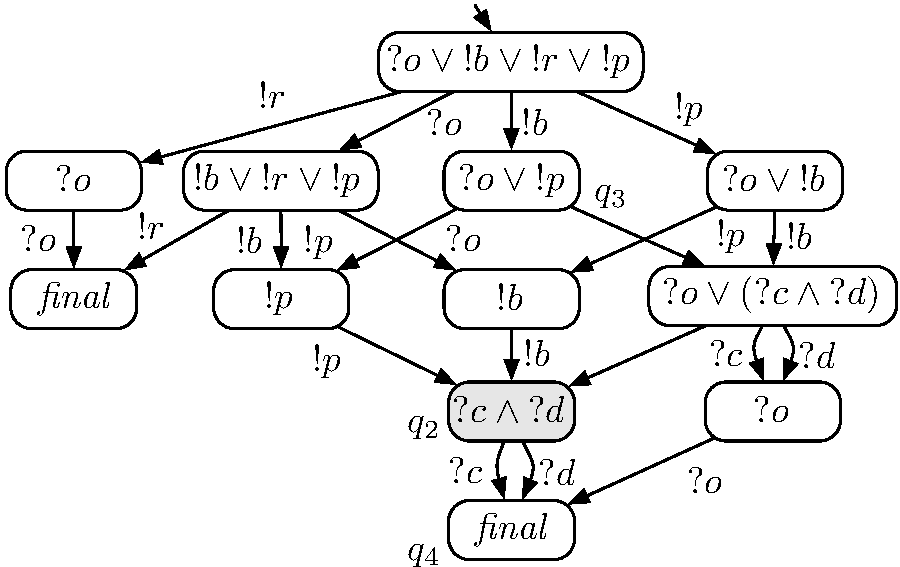
\includegraphics[scale=0.45]{correction/og}}}
\caption{The service automaton (a) modeling the customer from \autoref{fig:chor} and an operating guideline (b) of the composition of the travel agency and the airline service from \autoref{fig:chor}.}\label{fig:saog}
\end{figure}
%%%%%%%%%%%%%%%%%%%%%%%%%%%%%%%%%%%%%%%%%%%%%%%%%%%%%%%%%%%%%%%%%%%%%%%%%%%%%%

Beside the two corrected services in \autoref{fig:fix}, the operating guideline characterizes 2{,}302 additional (acyclic, deterministic, and $\tau$-free) strategies (up to isomorphism). This number can be derived from the connected subgraphs of the operating guideline and the labels which satisfy the annotated formulae. We use this number as an approximation, because the set of cyclic or nondeterministic partner services is usually infinite. Alhough each of these services is correct, we are interested in the service which is most similar to the incorrect customer service; that is, instead of iteratively checking an unreasonably high number of candidates, we shall define a similarity measure which exploits the operating guideline's compact representation to efficiently find the desired service of \autoref{fig:fix2}.





%%%%%%%%%%%%%%%%%%%%%%%%%%%%%%%%%%%%%%%%%%%%%%%%%%%%%%%%%%%%%%%%%%%%%%%%%%%%%%%
\section{Graph similarities}
\label{sect:graph}
%%%%%%%%%%%%%%%%%%%%%%%%%%%%%%%%%%%%%%%%%%%%%%%%%%%%%%%%%%%%%%%%%%%%%%%%%%%%%%%

Graph similarities are widely used in many fields of computer science, for example for pattern recognition~\cite{SanfeliuF_1983_smc}, semantic Web, document retrieval, or in bio informatics. Graph similarities are \emph{quantitative} measures and express the similarity of two graphs in a single value. To gain more insight in the reasons of (un)similarity, cost-based distance measures adapt the \emph{edit distance} known from string comparison~\cite{Levenshtein_1966_spd,WagnerF_1975_jacm} to compare labeled graphs~\cite{TsaiF_1979_smc,Bunke_1998_prl,Bunke_1997_prl}. They aim at finding the minimal number of modifications (\ie, adding, deleting, and modifying nodes or edges) needed to achieve a graph isomorphism.

Distance measures aiming at graph isomorphism have the drawback that they are solely rely on the \emph{structure} of the graphs. That is, they focus on the syntax of the graphs rather than their semantics. In case a graph (\eg, a service automaton) models the \emph{behavior} of a system, similarity of graphs should focus on similar behavior rather than on similar  structure. \Autoref{fig:edit} illustrates that structural and behavioral similarity are not related.

%%%%%%%%%%%%%%%%%%%%%%%%%%%%%%%%%%%%%%%%%%%%%%%%%%%%%%%%%%%%%%%%%%%%%%%%%%%%%%
\begin{figure}
\centering
\subfigure[$A_r$]{\makebox[0.3\textwidth]{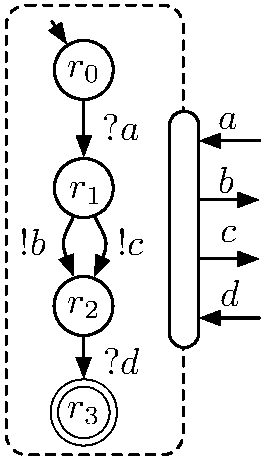
\includegraphics[scale=0.45]{correction/a2}}}
\subfigure[$A_s$]{\makebox[0.3\textwidth]{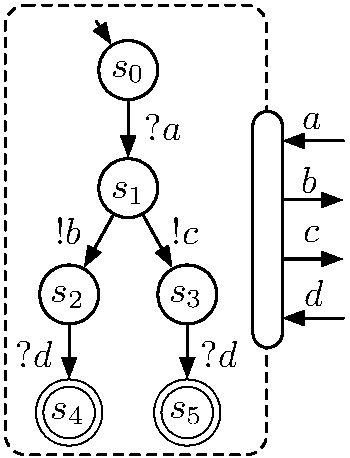
\includegraphics[scale=0.45]{correction/a1}}}
\subfigure[$A_t$]{\makebox[0.3\textwidth]{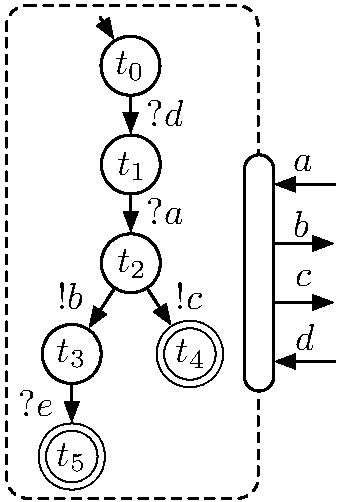
\includegraphics[scale=0.45]{correction/a3}}}
\caption{Service automata $A_r$ and $A_s$ simulate each other, but have an unsimilar structure. Service automata $A_s$ and $A_t$ have a  similar structure, but very different behaviors.}
\label{fig:edit}
\end{figure}
%%%%%%%%%%%%%%%%%%%%%%%%%%%%%%%%%%%%%%%%%%%%%%%%%%%%%%%%%%%%%%%%%%%%%%%%%%%%%%

\nomenclature[p]{$p$}{discount factor ($p\in [0,1]$)}%
\nomenclature[L]{$L(a,b)$}{label similarity ($a,b\in \E\cup\{\tau,\varepsilon\}$)}%
\nomenclature[e]{$\varepsilon$}{stuttering step}%
\citet{SokolskyKL_2006_tacas} address this problem (a similar approach is presented by~\citet{NejatiSCEZ_2007_icse}), motivated by finding computer viruses in a program. The idea is to compare the control flow graph of the program with a library of control flow graphs of known computer viruses and to warn if a certain threshold is exceeded. In that setting, a classical simulation relation as comparison between behavior is too strict, because two systems which are equal in all but one edge label \emph{behave} very similarly, but there exists no simulation relation between them. To this end, \citeauthor{SokolskyKL_2006_tacas} introduce a \emph{weighted quantitative simulation} function to compare states of two graphs. Whenever the two graphs cannot perform a transition with the same label, one graph performs a special stuttering step $\varepsilon$, which is similar to $\tau$-steps in stuttering bisimulation~\cite{Namjoshi_1997_fsttcs}. To ``penalize'' stuttering, a label similarity function assigns low similarity between $\varepsilon$ and any other label.

%%%%%%%%%%%%%%%%%%%%%%%%%%%%%%%%%%%%%%%%%%%%%%%%%%%%%%%%%%%%%%%%%%%%%%%%%%%%%%
\begin{definition}{Similarity function, discount factor}
For a set of message events $\E$ and a \define{stuttering event} $\varepsilon\notin\E$, a \define{similarity function} is a function $L:(\E\cup\{\tau,\varepsilon\})\times (\E\cup\{\tau,\varepsilon\})\rightarrow[0,1]$. A \define{discount factor} is a value $p\in [0,1]$.
\end{definition}
%%%%%%%%%%%%%%%%%%%%%%%%%%%%%%%%%%%%%%%%%%%%%%%%%%%%%%%%%%%%%%%%%%%%%%%%%%%%%%

A label similarity function assigns a value that expresses the similarity between the labels of the service automata under consideration. For example, $L({?a},{?b})$ describes the similarity of an ${?a}$-labeled transition of service automaton $A_{1}$ and a ${?b}$-labeled transition of service automaton $A_{2}$. Furthermore, a discount factor $p\in [0,1]$ describes the local importance of similarity compared with the similarity of successor states. This discount ``smoothens'' the simulation results by not only considering local similarity (\eg, by comparing the similarity of labels of outgoing edges), but also the future similarity (\ie, the similarity of successor states). Both $L$ and $p$ will influence the upcoming definitions to calculate similarities and edit distances. Their values can be chosen freely to adjust the result of the similarity algorithm. The concrete choice of the parameters needs further empirical investigation and is therefore not considered here.

The following definition determines the similarity of two states of $A_1$ and $A_2$ by choosing which labels should synchronize. This evaluation is influenced by the label similarity function $L$ and the recursive similarity of the successor states. The label $\varepsilon$ further allows one service automaton to stutter rather than to synchronize.

%%%%%%%%%%%%%%%%%%%%%%%%%%%%%%%%%%%%%%%%%%%%%%%%%%%%%%%%%%%%%%%%%%%%%%%%%%%%%%%
\begin{definition}{Weighted quantitative simulation, \cite{SokolskyKL_2006_tacas}}\label{def:wwqs}%
For $i\in\{1,2\}$, let $A_{i}=[Q_{i},q_{0_{i}},{\shortrightarrow}_{i},\Omega_{i},\mathcal{P}_{i}]$ be service automata.
A \define{weighted quantitative simulation} is a function $S:Q_{1}\times Q_{2}\rightarrow [0,1]$, such that:
\begin{equation*}
S(q_{1},q_{2}) := \begin{cases}
1, & \text{if $q_{1}\not\xrightarrow{}_{1}{}$}, \\
(1-p)+p \cdot\max\Bigl(W_{1}(q_{1},q_{2}),\displaystyle\frac{1}{n}\cdot W_{2}(q_{1},q_{2})\Bigr), & \text{otherwise,}
\end{cases}\\
\end{equation*}
\begin{equation*}
W_{1}(q_{1},q_{2}):=\max_{q_{2}\xrightarrow{b}_2 q_{2}'} \Bigl( L(\varepsilon,b)\cdot S(q_{1},q_{2}') \Bigr),
\end{equation*}
\begin{equation*}
W_{2}(q_{1},q_{2}):=\!\!\sum_{q_{1}\xrightarrow{a}_1 q_{1}'}\!\!\max\left(L(a,\varepsilon)\cdot S(q_{1}',q_{2}), \max_{q_{2}\xrightarrow{b}_2 q_{2}'} \Bigl(L(a,b)\cdot S(q_{1}',q_{2}')\Bigr) \right),
\end{equation*}
and $n$ is the number of edges leaving $q_{1}$. The weighted quantitative simulation between $A_{1}$ and $A_{2}$ is defined as $S(q_{0_{1}},q_{0_{2}})$.
\end{definition}
%%%%%%%%%%%%%%%%%%%%%%%%%%%%%%%%%%%%%%%%%%%%%%%%%%%%%%%%%%%%%%%%%%%%%%%%%%%%%%%

The weighted quantitative simulation function $S$ recursively compares the states from the two service automata and finds the maximal similar edges. Thereby, $W_{1}$ describes the similarity gain by stuttering of service automaton~$A_{1}$ on the one hand, and $W_{2}$ the tradeoff between simultaneous transitions of~$A_{1}$ and $A_{2}$ and stuttering of service automaton $A_{2}$ on the other hand. A sink state of $A_{1}$ (\ie, a state without successors) has a maximal similarity with any state of $A_{2}$, because there are no obligations for $A_{2}$ to simulate this state.

\citet{SokolskyKL_2006_tacas} proved that a unique fixed point for $S$ exists and that $S$ generalizes classical simulation: If $A_{1}$ is simulated by $A_{2}$, then $S(q_{0_{1}},q_{0_{2}})=1$, and if $A_{1}$ is not simulated by $A_{2}$, then $S(q_{0_{1}},q_{0_{2}})<1$. In addition the authors provided a linear programming algorithm to calculate the weighted quantitative simulation for arbitrary finite state automata. We adjusted the definitions of \cite{SokolskyKL_2006_tacas} to service automata. The original definitions are based on labeled directed graphs and additionally take node labels and similarities between node labels into account. This is not required in the context of this chapter, but may be exploited in the future to further refine the results.


\paragraph{Example.}

Consider the service automata in \autoref{fig:edit} and assume a discount factor $p=0.7$ and a label similarity function $L$, which assigns $1.0$ to equal labels and $0.5$ to any other label pair. Then $S({r_{0}},{s_{0}})=1.0$ (the weighted quantitative simulation is a generalization of the classical simulation) and $S({s_{0}},{t_{0}})= 0.589975$ which indicates the differences in the behaviors of $A_s$ and $A_t$. This latter result can be calculated as follows (only the local maxima are shown):
\begin{flalign*}
\qquad S(s_0,t_0) &= (1-p)�+ p\cdot L({\varepsilon},{?d})\cdot S(s_0,t_1)= 0.589975 \\
S(s_0,t_1) &= (1-p) + p\cdot L({?a},{?a}) \cdot S(s_1,t_1)= 0.8285 \\
S(s_1,t_1) &= (1-p) + \smash{\textstyle\frac{p}{2}}\cdot \bigl( L({!b},{!b})\cdot S(s_2,t_4) + L({!c},{!c})\cdot S(s_3,t_4) \bigr) = 0.755 \\
S(s_2,t_3) &= (1-p) + p\cdot L({?d},{\sync e})\cdot S(s_4,t_5) =  0.65\\
S(s_3,t_4) &= (1-p) + p\cdot L({?d},{\varepsilon})\cdot S(s_5,t_4) =  0.65�\\
S(s_4,t_5) &= 1& \\
S(s_5,t_4) &= 1&
\end{flalign*}
Intuitively, \autoref{def:wwqs} can be seen as a system of equations, having the values of $S$ as variables. Some variables (\eg, $S(s_0,t_0)$) depend on other variables, whereas other variables (\eg, $S(s_5,t_4)$) do not. As illustration, consider the definition of $S(s_{0},t_{0})$:
\begin{flalign*}
\text{\fbox{$S(s_0,t_0)$}} =\, &(1-p)+p\cdot\max \bigl( \overbrace{L(\varepsilon,{?d})\cdot \text{\fbox{$S(s_0,t_1)$}}}^{W_{1}(s_{0},t_{0})},\\
&\frac{1}{n}\cdot (\underbrace{\max( L({?a},\varepsilon)\cdot \text{\fbox{$S(s_1,t_0)$}},\; L({?a},{?d})\cdot \text{\fbox{$S(s_1,t_1)$}} )}_{W_{2}(s_{0},t_{0})}\bigr)
\end{flalign*}
The framed values represent variables of the equation system: the value of $S(s_0,t_0)$ depends on the values of $S(s_0,t_1)$, $S(s_1,t_0)$, and $S(s_1,t_1)$.





%%%%%%%%%%%%%%%%%%%%%%%%%%%%%%%%%%%%%%%%%%%%%%%%%%%%%%%%%%%%%%%%%%%%%%%%%%%%%%%
\section{A matching-based edit distance}\label{sect:combine}
%%%%%%%%%%%%%%%%%%%%%%%%%%%%%%%%%%%%%%%%%%%%%%%%%%%%%%%%%%%%%%%%%%%%%%%%%%%%%%%

The weighted quantitative simulation of \autoref{def:wwqs} can be used as a similarity measure for service automata or operating guidelines, but has two drawbacks: First, it is not an edit distance. It calculates a single value which expresses the similarity between the service automata, but gives no information about the modification actions needed to \emph{achieve} simulation. Second, it does not take formulae of the operating guideline into account. Therefore, even a perfect similarity (which is closely related to structural matching) between a service automaton and an operating guideline would not guarantee compatibility as the example of \autoref{fig:saog} demonstrates: The service automaton of the customer is structurally matched by the operating guideline but the overall choreography deadlocks.




%%%%%%%%%%%%%%%%%%%%%%%%%%%%%%%%%%%%%%%%%%%%%%%%%%%%%%%%%%%%%%%%%%%%%%%%%%%%%%%
\subsection*{Simulation-based edit distance}

Before we consider the operating guideline's formulae, we show how the similarity metric of \autoref{def:wwqs} (\ie, the result of the algorithm of~\cite{SokolskyKL_2006_tacas}) can be transformed into an edit distance.

Given two states $q_{1}$ and $q_{2}$ of two service automata $A_1$ and $A_2$, \autoref{def:wwqs} determines the similarity $S(q_1,q_2)$ by choosing pairs of labels of transitions leaving $q_1$ and $q_2$, respectively. Each pair of labels $[a,b]$ with \smash{$q_1\xrightarrow{a}_1 q_1'$} and \smash{$q_2\xrightarrow{b}_2 q_2'$} determines successor states whose similarity is then recursively determined by $S(q_1',q_2')$. The similarity of $q_1$ and $q_2$ is then calculated by locally maximizing the successor state's similarity. From \autoref{def:wwqs}, we can derive a graph consisting of the state pairs as nodes and the chosen label pairs as transitions:

%\enlargethispage*{2\baselineskip}

%%%%%%%%%%%%%%%%%%%%%%%%%%%%%%%%%%%%%%%%%%%%%%%%%%%%%%%%%%%%%%%%%%%%%%%%%%%%%%%
\begin{definition}{Synchronization graph}\label{corr:def:sync}%
\nomenclature{$\odot$}{synchronization of service automata}%
Let $A=[Q_{A},q_{0_{A}},{\shortrightarrow}_{A},\Omega_{A},\mathcal{P}_A]$ and $B=[Q_{B},q_{0_{B}},{\shortrightarrow}_{B},\Omega_{B},\mathcal{P}_B]$ be service automata. The \define{synchronization graph} of $A$ and~$B$ is the tuple $A\odot B=[Q,q_0,{\shortrightarrow}]$ consisting of
\begin{myitemize}
\item $Q:=Q_A\times Q_B$,
\item $q_0 := [q_{0_A}, q_{0_B}]$,
\item ${\shortrightarrow}$, containing exactly the following elements:
\begin{myitemize}
\item $[q_A,q_B]\xrightarrow{[x,y]}�[q_A',q_B']$ iff $q_A\xrightarrow{x}_A q_A'$ and $q_B\xrightarrow{y}_B q_B'$, 
\item $[q_A,q_B]\xrightarrow{[x,\varepsilon]}�[q_A',q_B]$ iff $q_A\xrightarrow{x}_A q_A'$, and 
\item $[q_A,q_B]\xrightarrow{[\varepsilon,y]}�[q_A,q_B']$ iff $q_B\xrightarrow{y}_B q_B'$.
\end{myitemize}
\end{myitemize}
\end{definition}
%%%%%%%%%%%%%%%%%%%%%%%%%%%%%%%%%%%%%%%%%%%%%%%%%%%%%%%%%%%%%%%%%%%%%%%%%%%%%%%

Intuitively, this graph has the variables of the previously motivated equation systems as nodes. A transition \smash{$[q_{A},q_{B}] \xrightarrow{[x,y]} [q_{A}',q_{B}']$} states that the value of $S(q_{A},q_{B})$ depends on the value of $L(x,y)\cdot S(q_{A}',q_{B}')$.

%%%%%%%%%%%%%%%%%%%%%%%%%%%%%%%%%%%%%%%%%%%%%%%%%%%%%%%%%%%%%%%%%%%%%%%%%%%%%%
\begin{figure}
\centering
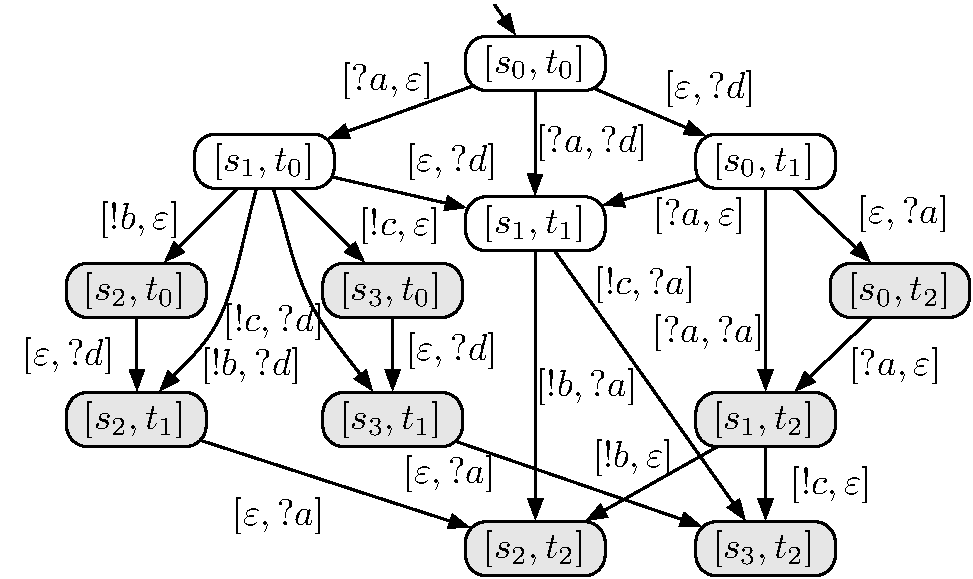
\includegraphics[scale=0.4]{correction/sg}
\caption{Part of the synchronization graph $A_s \odot A_t$.}\label{fig:correction:sg}
\end{figure}
%%%%%%%%%%%%%%%%%%%%%%%%%%%%%%%%%%%%%%%%%%%%%%%%%%%%%%%%%%%%%%%%%%%%%%%%%%%%%%


\paragraph{Example.}

\Autoref{fig:correction:sg} depicts the synchronization graph of the service automata $A_s$ and $A_t$ (cf.~\autoref{fig:edit}) to the depth of 2. That is, we do not depict all successor states of the shaded states.

\medskip

The synchronization graph can be seen as the search space for the optimal result  calculated by \autoref{def:wwqs}. As stated before, we are not just interested in a single value expressing the similarity of two service automata, but in instructions how to change a service automaton to achieve a structural matching. As intermediate result, we restrict the labels of the synchronization graph as follows: from the determined label pairs $[x,y]$ only the second part, $y$, is kept. Thereby, $\varepsilon$-labels are replaced by $\tau$.

%%%%%%%%%%%%%%%%%%%%%%%%%%%%%%%%%%%%%%%%%%%%%%%%%%%%%%%%%%%%%%%%%%%%%%%%%%%%%%%
\begin{definition}{Synchronization graph restriction}\label{corr:def:res}%
Let $A=[Q_{A},q_{0_{A}},{\shortrightarrow}_{A},\Omega_{A},\mathcal{P}_A]$ and $B=[Q_{B},q_{0_{B}},{\shortrightarrow}_{B},\Omega_{B},\mathcal{P}_B]$ be service automata and $A\odot B=[Q_{AB},q_{0_{AB}},{\shortrightarrow}_{AB}]$ their synchronization graph. We define the \define{restriction} of $A\odot B$ to $B$ as the service automaton $(A\odot B)_{|B}:=[Q_{AB},q_{0_{AB}},{\shortrightarrow},\Omega,\mathcal{P}_B]$ with:
\begin{myitemize}
\item $\Omega:= \Omega_A\times Q_B$ and
\item ${\shortrightarrow}$ containing exactly the following elements:
\begin{myitemize}
\item $[q,y,q']\in {\shortrightarrow}$ iff $[q,[x,y],q']\in {\shortrightarrow}_{AB}$ and $y\neq\varepsilon$ and
\item $[q,\tau,q']\in {\shortrightarrow}$ iff $[q,[x,y],q']\in {\shortrightarrow}_{AB}$ and $y=\varepsilon$.
\end{myitemize}
\end{myitemize}
\end{definition}
%%%%%%%%%%%%%%%%%%%%%%%%%%%%%%%%%%%%%%%%%%%%%%%%%%%%%%%%%%%%%%%%%%%%%%%%%%%%%%%

The restriction of the synchronization graph $A\odot B$ to the labels of the interface of service automaton $B$ yields a service automaton \mbox{$(A\odot B)_{|B}$}, which structurally matches $B$. Additionally, $[q_A,q_B]$ is a final state of $(A\odot B)_{|B}$ iff $q_A$ is a final state of $A$. Although final states are not considered by structural matching, they are later required to evaluate the operating guideline's formulae.

From the definition of structural matching (cf.~\autoref{def:smatching}), \autoref{corr:def:sync}, and \autoref{corr:def:res}, we can derive the following result:

%%%%%%%%%%%%%%%%%%%%%%%%%%%%%%%%%%%%%%%%%%%%%%%%%%%%%%%%%%%%%%%%%%%%%%%%%%%%%%%
\begin{corollary}{Restriction structurally matches.}\label{corr:cor:match}%
Let $A=[Q_{A},q_{0_{A}},{\shortrightarrow}_{A},\Omega_{A},\mathcal{P}_A]$ and $B=[Q_{B},q_{0_{B}},{\shortrightarrow}_{B},\Omega_{B},\mathcal{P}_B]$ be service automata.\\ Then $(A\odot B)_{|B}$ structurally matches $B$.
\end{corollary}
%%%%%%%%%%%%%%%%%%%%%%%%%%%%%%%%%%%%%%%%%%%%%%%%%%%%%%%%%%%%%%%%%%%%%%%%%%%%%%%

%%%%%%%%%%%%%%%%%%%%%%%%%%%%%%%%%%%%%%%%%%%%%%%%%%%%%%%%%%%%%%%%%%%%%%%%%%%%%%
\begin{figure}
\centering
\subfigure[subgraph of $A_s\odot A_t$\label{fig:synca}]{\makebox[0.45\textwidth]{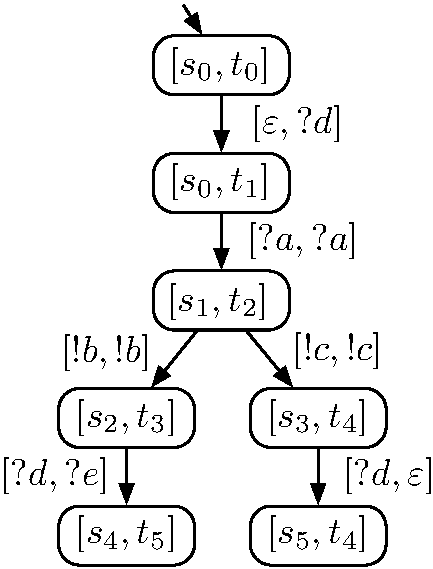
\includegraphics[scale=0.45]{correction/sync}}}
\subfigure[restriction $(A_s\odot A_t)_{|A_t}$\label{fig:syncb}]{\makebox[0.45\textwidth]{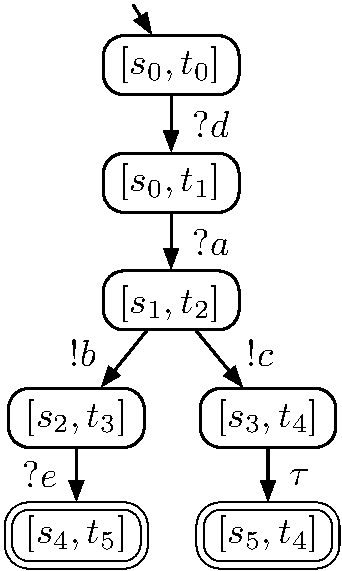
\includegraphics[scale=0.45]{correction/rsync}}}
\caption{Subgraph of the synchronization graph $A_s\odot A_t$ (a) and  its restriction to $(A_s\odot A_t)_{|A_t}$ (b).}
\label{fig:sync}\bigskip
\end{figure}
%%%%%%%%%%%%%%%%%%%%%%%%%%%%%%%%%%%%%%%%%%%%%%%%%%%%%%%%%%%%%%%%%%%%%%%%%%%%%%

\Autoref{def:wwqs} choses for each pair of states $[q_a,q_b]$\,---\,or, for each state of the synchronization graph\,---\,those successors states where the local similarity is maximal with respect to the label similarity function $L$. This choice implicitly defines a subgraph of the synchronization graph, because not every state and label pair is part of an optimal solution.


\paragraph{Example.}

The application of \autoref{def:wwqs} to calculate $S(s_0,t_0)$,\,---\,the weighted quantitive simulation between the service automata $A_{s}$ and $A_{t}$ of \autoref{fig:edit}\,---\,implicitly defines a subgraph of the synchronization graph $A_s\odot A_t$, which is depicted in \autoref{fig:synca}. Applying \autoref{corr:def:res},  this graph can be restricted to $(A_s\odot A_t)_{|A_t}$ (cf.~\autoref{fig:syncb}), which by \autoref{corr:cor:match} is structurally matched by $A_t$.

\smallskip

The subgraph of $A\odot B$ is implicitly defined by \autoref{def:wwqs} and can be used as an edit distance as follows: Each transition is labeled by a pair of a label of $A$ and a label $B$. In addition, $\varepsilon$ can occur to model stuttering. A pair $[a,b]$ can then be interpreted as an \emph{edit action}; that is, as instructions to change the label $a$ to $b$. Additionally, a pair $[\varepsilon,b]$ demands adding a $b$-labeled transition, whereas $[a,\varepsilon]$ demands the removal of the $a$-label and replacing it by $\tau$. The latter would correspond to the deletion of a letter in the setting of string manipulation. \Autoref{tab:edit} lists these edit actions.

%%%%%%%%%%%%%%%%%%%%%%%%%%%%%%%%%%%%%%%%%%%%%%%%%%%%%%%%%%%%%%%%%%%%%%%%%%%%%%
\begin{table}
\caption{Deriving edit actions from transition pairs of Def.~\ref{def:wwqs}.}
\centering \footnotesize%\small
\begin{tabular*}{\textwidth}{@{\extracolsep{\fill}}cccc}
\toprule
transition of $A_{1}$ & transition of $A_{2}$ & resulting edit action & similarity \\ \midrule
${a}$ & ${a}$ & keep label ${a}$ & $L({a},{a})$ \\
${a}$ & ${b}$ & modify label from ${a}$ to ${b}$ & $L({a},{b})$ \\
${a}$ & $\varepsilon$ (stutter) & change transition label ${a}$ to $\tau$ & $L({a},{\varepsilon})$ \\
$\varepsilon$ (stutter) & ${a}$ & insert transition with label ${a}$ & $L({\varepsilon},{a})$ \\ \bottomrule
\end{tabular*}
\label{tab:edit}
\end{table}
%%%%%%%%%%%%%%%%%%%%%%%%%%%%%%%%%%%%%%%%%%%%%%%%%%%%%%%%%%%%%%%%%%%%%%%%%%%%%%

These edit actions define \emph{basic edit actions} whose similarity is determined by the edge similarity function $L$. To simplify the representation of a large number of edit actions, the basic edit actions may be grouped to macros to express more complex operations such as swapping or moving of edges and nodes, duplicating of subgraphs, or partial unfolding of loops.

%%%%%%%%%%%%%%%%%%%%%%%%%%%%%%%%%%%%%%%%%%%%%%%%%%%%%%%%%%%%%%%%%%%%%%%%%%%%%%
\begin{figure}
\centering
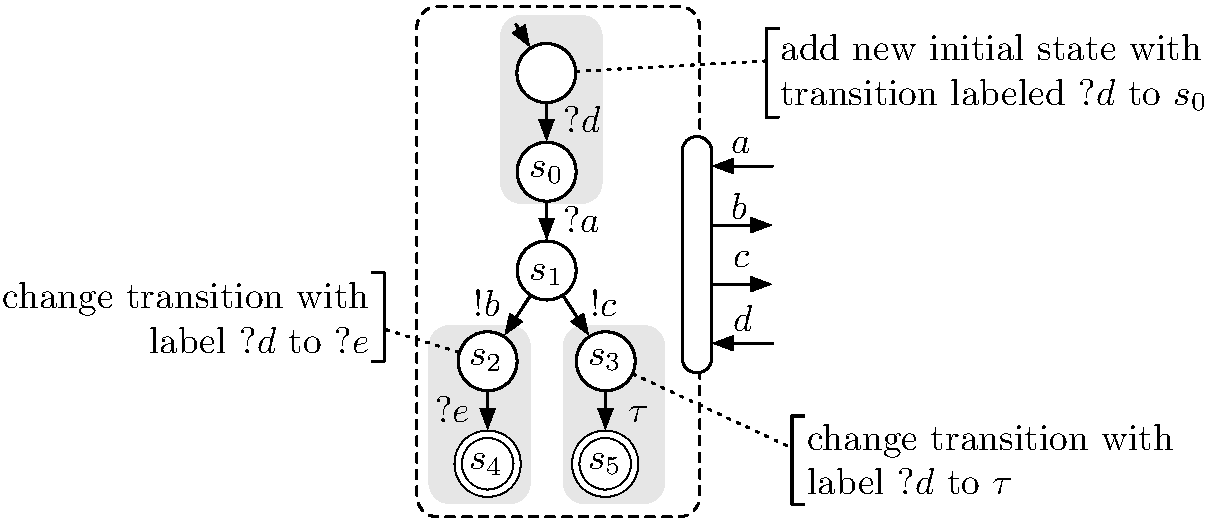
\includegraphics[scale=0.45]{correction/fix}
\caption{Simulation-based edit distance between $A_s$ and $A_t$.}
\label{fig:corrfix}
\end{figure}
%%%%%%%%%%%%%%%%%%%%%%%%%%%%%%%%%%%%%%%%%%%%%%%%%%%%%%%%%%%%%%%%%%%%%%%%%%%%%%


\paragraph{Example.}

With \autoref{tab:edit}, we can derive from \autoref{fig:synca} edit actions how to change $A_{s}$ to $(A_s\odot A_t)_{|A_t}$. \Autoref{fig:corrfix} depicts these edit actions. They show how the service automaton $A_s$ needs to be changed to be structurally matched by $A_t$. We thereby do not explicitly annotate the keeping of edge labels.




%%%%%%%%%%%%%%%%%%%%%%%%%%%%%%%%%%%%%%%%%%%%%%%%%%%%%%%%%%%%%%%%%%%%%%%%%%%%%%%
\subsection*{Combining formula satisfaction and graph similarity}

So far, we defined a simulation-based edit distance which, given two service automata $A_{1}$ and $A_{2}$, provides minimal editing steps to change $A_{1}$ such that it is simulated by $A_{2}$. Coming back to the correction scenario motivated in \autoref{sect:corr:mot}, $A_{1}$ has the role of an incorrect service and $A_{2}$ the role of a correct service. However, we are interested in the similarity to \emph{all} possible correct services characterized by an operating guideline $B^{\varphi}$. In the remainder of this section, we shall extend the simulation-based edit distance accordingly.

\medskip

The simulation-based edit distance does not respect the formulae of operating guidelines. One possibility to achieve a matching would be to first calculate the most similar simulating service using the edit distance for \autoref{def:wwqs} and then to add and remove all nodes and edges necessary in a second step. However, the insertion of nodes would not determine the most similar partner service, because this may result in suboptimal solutions as \autoref{fig:sim} illustrates. The service automaton (a) is structurally matched by the operating guideline (b), but the formula ${?c}\wedge {?d}\wedge {?e}$ is not satisfied. Adding two states and transitions to (a) fixes this (c). However, changing the edge label of (a) from ${!a}$ to ${!b}$ also achieves matching, but only requires a single edit action~(d).

%%%%%%%%%%%%%%%%%%%%%%%%%%%%%%%%%%%%%%%%%%%%%%%%%%%%%%%%%%%%%%%%%%%%%%%%%%%%%%
\begin{figure}
\centering
{}\hfill\subfigure[service automaton\label{fig:corr:sasub}]{\makebox[0.4\textwidth]{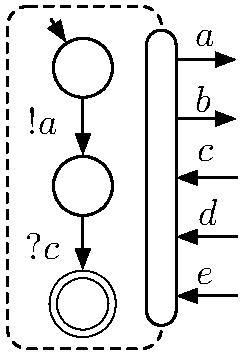
\includegraphics[scale=0.45]{correction/sim1}}}\hfill
\subfigure[operating guideline\label{fig:corr:ogsub}]{\makebox[0.4\textwidth]{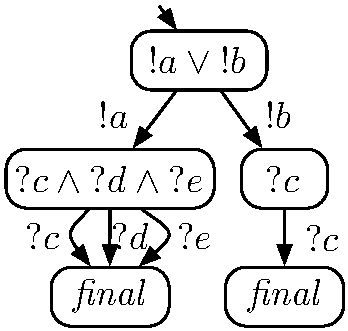
\includegraphics[scale=0.45]{correction/sim2}}}\hfill\\\vspace{-0.5em}
{}\hfill\subfigure[suboptimal edit distance]{\makebox[0.4\textwidth]{\hspace{4em}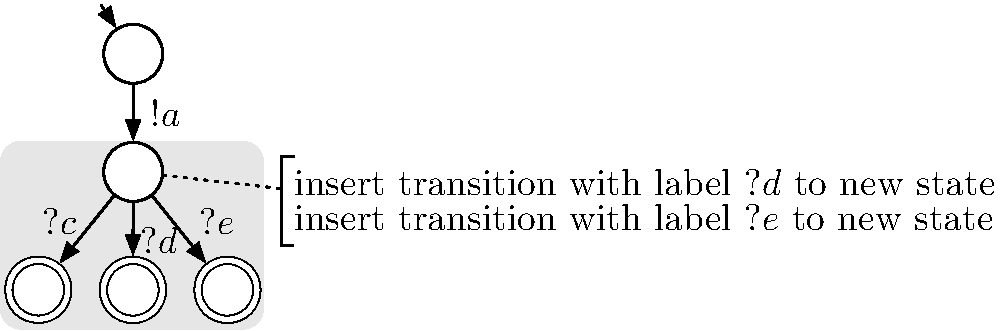
\includegraphics[scale=0.45]{correction/sim3}}} \hfill
\subfigure[optimal edit distance]{\makebox[0.4\textwidth]{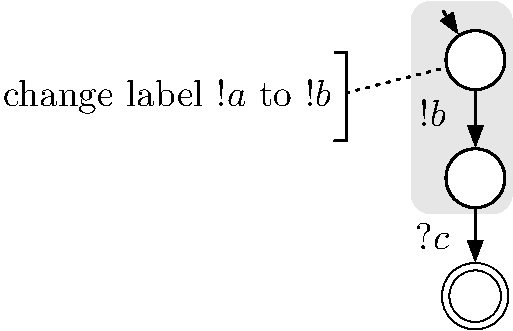
\includegraphics[scale=0.45]{correction/sim4}}}\hfill
\caption{Adding states to a simulating service automaton may yield suboptimal results.}
\label{fig:sim}
\end{figure}
%%%%%%%%%%%%%%%%%%%%%%%%%%%%%%%%%%%%%%%%%%%%%%%%%%%%%%%%%%%%%%%%%%%%%%%%%%%%%%

Because of the suboptimal results achieved through a-posteriori formula satisfaction by node insertion, we need to modify the algorithm of~\cite{SokolskyKL_2006_tacas} to check any formula-fulfilling \emph{subset} of outgoing transitions. For the remainder of this chapter, we pose the following restrictions on the service automaton and the operating guideline under consideration and assume $A=[Q_{A},q_{0_{A}},{\shortrightarrow}_{A},\Omega_{A},\mathcal{P}_{A}]$ is a service automaton and $B^\varphi=[Q_{B},q_{0_{B}},{\shortrightarrow}_{B},\mathcal{P}_{B},\varphi]$ is an operating guideline following these restrictions that we shall discuss in \autoref{sect:conclusion}.

\begin{niceenumerate}
\item The service automaton $A$ is \emph{deterministic}. Hence, we can treat the transition relation~$\shortrightarrow_A$ as a function and can write \smash{${\shortrightarrow_A}(q_A,x)=q_A'$} instead of \smash{$q_{A}\xrightarrow{x}q_{A}'$}.
\item Both the service automaton $A$ and the operating guideline $B^{\varphi}$ are \emph{acyclic}. For the operating guideline, we do not consider the empty node $q=\emptyset$ as this node models unreachable behavior which should not be taken into account when correcting a service with respect to a concrete service composition.
\item The final states of the service automaton $A$ must be \emph{sink states}; that is, $q\xrightarrow{x}_{A}q'$ implies $q\notin\Omega_{A}$ for all $q\in Q_{A}$. Furthermore, $\mathit{final}$ is assumed to only occur in sink states of the operating guideline.
\end{niceenumerate}

We need to define additional concepts to include formula satisfaction and to cover the implicit characterization of multiple services by a single operating guideline. We first define label permutations as means to enumerate all the possibilities of changes of the service automaton's labels that are required to satisfy an operating guideline's annotated formula.

%%%%%%%%%%%%%%%%%%%%%%%%%%%%%%%%%%%%%%%%%%%%%%%%%%%%%%%%%%%%%%%%%%%%%%%%%%%%%%%
\begin{definition}{Satisfying label set}\label{def:corrsat}%
Let $B^\varphi$ be as above and let $q_{B}\in Q_{B}$. We define the assignment $\beta':Q_B\times(\E\cup\{\final\})\rightarrow\{\mathit{true},\mathit{false}\}$ as follows:
$$\beta'(q_{B},p):=\begin{cases}
\mathit{true}\text{,}&\text{if $p\in \lab(q_{B})$,}\\
\mathit{true}\text{,}&\text{if $p=\final$,}\\
\mathit{false}\text{,}&\text{otherwise}.
\end{cases}$$
A state $q_{B}\in Q_{B}$ \define{models} a formula $\varphi$ (denoted $q_{B}\models'\varphi$) iff $\varphi$ evaluates to $\mathit{true}$ under the assignment $\beta'(q_{B},\varphi)$. We thereby assume the standard semantics for the Boolean operators $\wedge$, $\vee$, and $\neg$.

Let \smash{$\mathop{Sat}(\varphi(q_{B})):=\{l \in \lab(q_{B}) \mid l\models'\varphi(q_B) \}$} be the set of all sets of labels of transitions leaving $q_{B}$ that satisfy formula $\varphi$ of state~$q_{B}$.
\end{definition}
%%%%%%%%%%%%%%%%%%%%%%%%%%%%%%%%%%%%%%%%%%%%%%%%%%%%%%%%%%%%%%%%%%%%%%%%%%%%%%%

Compared with \autoref{def:assignment}, we evaluate the operating guideline's formulae independent of a service automaton. Thereby, we only take the operating guideline's structure into account. The intuition is that the operating guideline characterizes by itself all correct candidates for the correction (cf.\ \autoref{fig:space}). Final states and the $\mathit{final}$ predicate do not need to be considered, because we assumed final states to be sink states. The set $\mathop{Sat}$ consists of all sets of labels which satisfy a state's formula. To match with this state, a service automaton's state must have outgoing edges with exactly these labels.


\paragraph{Example.}

Consider the operating guideline in \autoref{fig:corrog}: It holds: $\mathop{Sat}(\varphi({q_{2}}))=\{ \{{?c},{?d}\} \}$, because the formula ${?c}\wedge{?d}$ has only this satisfying assignment;\break $\mathop{Sat}(\varphi({q_{3}}))=\{ \{{?o}\},  \{{!p}\},$ $ \{{?o},{!p}\} \}$, because the formula ${?o}\vee{!p}$ has these three satisfying assignments; and $\mathop{Sat}(\varphi({q_{4}}))=\emptyset$, because $q_{4}$ is a sink state (\ie, has no outgoing transitions) and is annotated with $\mathit{final}$.

\smallskip

The calculation of the weighted quantitative simulation (cf.\ \autoref{def:wwqs}) between two service automata $A_{1}$ and $A_{2}$ is based on pairs of transition labels (one for each service automaton). These pairs of labels are then used to derive the simulation-based edit distance (cf.\ \autoref{tab:edit}). The pairs were determined by the transition relation of the service automata. To determine the similarity between a service automaton $A$ and an operating guideline $B^{\varphi}$, this is not sufficient. Instead, we need to consider the transition relation of $A$ and the satisfying label sets of~$B^{\varphi}$.\pagebreak

%%%%%%%%%%%%%%%%%%%%%%%%%%%%%%%%%%%%%%%%%%%%%%%%%%%%%%%%%%%%%%%%%%%%%%%%%%%%%%%
\begin{definition}{Label permutation}\label{def:corrsat2}%
Let $A$ and $B^\varphi$ be as above, and let $q_{A}\in Q_{A}$ and $q_{B}\in Q_{B}$. For $\beta\in\mathop{Sat}(\varphi(q_{B}))$, define $\mathop{perm}(q_{A},q_{B},\beta)\subset \bigl((\E \cup\{\varepsilon\}) \times (\E \cup\{\varepsilon\})\bigr)$ to be a \define{label permutation} of $q_{A}$, $q_{B}$ and $\beta$ such that:
\begin{enumerate}%[(a)]
\item if \smash{$q_{A}\xrightarrow{a}_Aq_{A}'$}, then $(a,c)\in\mathop{perm}(q_{A},q_{B},\beta)$ for some label $c\in\beta\cup\{\varepsilon\}$,
\item if \smash{$q_{B}\xrightarrow{b}_Bq_{B}'$} and $b\in\beta$, then $(d,b)\in\mathop{perm}(q_{A},q_{B},\beta)$ for some label $d\in \E\cup\{\varepsilon\}$,
\item $(\varepsilon,\varepsilon)\notin \mathop{perm}(q_{A},q_{B},\beta)$, and
\item if $(a,b)\in \mathop{perm}(q_{A},q_{B},\beta)$, then $(a,c)$, $(d,b)\notin \mathop{perm}(q_{A},q_{B},\beta)$ for all labels $c\neq b$ and $d\neq a$. % $c\in\beta\cup\{\varepsilon\}$ and all labels $d\in \E\cup\{\varepsilon\}$.
\end{enumerate}
Define \smash{$\mathop{Perms}(q_{A},q_{B},\beta)\subseteq 2^{(\E \cup\{\varepsilon\}) \times (\E \cup\{\varepsilon\})}$} to be the set of all label permutations of $q_{A}$, $q_{B}$, and~$\beta$.
\end{definition}
%%%%%%%%%%%%%%%%%%%%%%%%%%%%%%%%%%%%%%%%%%%%%%%%%%%%%%%%%%%%%%%%%%%%%%%%%%%%%%%

Intuitively, each outgoing edge of $q_{A}$ is mapped onto at most one outgoing edge of $q_{B}$ such that we can derive edit actions from this mapping to achieve a structural matching between $q_{A}$ and $q_{B}$. Specifically, the set $\mathop{Perms}$ consists of all permutations of outgoing edges of two states. In a permutation, each outgoing edge of a state of the service automaton has to be present as first element of a pair~(1), each outgoing edge of a state of the operating guideline that is part of the label set~$\beta$ has to be present as second element of a pair~(2). As the number of outgoing edges of the states may differ, $\varepsilon$-labels can occur in the pairs, but no pair $(\varepsilon,\varepsilon)$ is allowed~(3), because we want to exclude simultaneous stuttering. Finally, each edge is only allowed to occur once in a pair~(4). This definition exploits the assumption that $A$ is deterministic.

\paragraph{Example.}

For state ${q_{1}}$ of the service automaton in \autoref{fig:corsa}, state $q_{2}$ of the operating guideline in \autoref{fig:corrog}, and $\beta=\{{?c},{?d}\}$, one of the permutations in $\mathop{Perms}({q_{1}},{q_{2}},\beta)$ is $\{({?c},{?c}), (\varepsilon,{?d})\}$. Two other permutation are $\{({?c},{?d}), (\varepsilon,{?c})\}$ and $\{({?c},\varepsilon), (\varepsilon,{?c}), (\varepsilon,{?d})\}$. The permutations can be interpreted just like the label pairs of the simulation edit distance: $({?c},{?c})$ describes keeping the label ${?c}$, $({?c},{?d})$ describes changing label ${?c}$ to ${?d}$, and $(\varepsilon,{?d})$ the insertion of a ${?d}$-labeled transition.

\smallskip

The insertion and deletion has to be adapted to avoid incorrect or suboptimal results (cf.~\autoref{fig:sim}). This is achieved by taking the structure as well as the formulae into account. The following definition relies on the fact that both $A$ and $B^{\varphi}$ are acyclic and deterministic, and that their final states are sink states.

%%%%%%%%%%%%%%%%%%%%%%%%%%%%%%%%%%%%%%%%%%%%%%%%%%%%%%%%%%%%%%%%%%%%%%%%%%%%%%%
\begin{definition}{Subgraph insertion, subgraph deletion}
Let $A$ and $B^\varphi$ be as above, $q_A\in Q_A$, and $q_B\in Q_B$. We define
\begin{align*}
\mathop{ins}(q_{B})&=
\begin{cases}
1,&\text{if $q_{B}\not\xrightarrow{}_B$,}\\
\displaystyle (1-p)+\max_{\beta\in\mathop{Sat}(\varphi(q_{B}))}\frac{p}{|\beta|}\cdot\sum_{b\in\beta}L(\varepsilon,b)\cdot\mathop{ins}({\shortrightarrow_B}(q_{B},b)),&\text{otherwise,}
\end{cases}\\
%\end{equation*}
%\begin{equation*}
\mathop{del}(q_{A})&=
\begin{cases}
1,&\text{if $q_{A}\in \Omega_{A}$,}\\
\displaystyle (1-p)+\frac{p}{n}\cdot\sum_{q_{A}\xrightarrow{a}_A q_{A}'}L(a,\varepsilon)\cdot\mathop{del}(q_{A}'),&\text{otherwise,}
\end{cases}
\end{align*}
where $n$ is the number of outgoing edges of $q_{A}$.
\label{def:insdel}
\end{definition}
%%%%%%%%%%%%%%%%%%%%%%%%%%%%%%%%%%%%%%%%%%%%%%%%%%%%%%%%%%%%%%%%%%%%%%%%%%%%%%%

Function $\mathop{ins}(q_{B})$ calculates the insertion cost of the optimal (acyclic) subgraph of the operating guideline $B^\varphi$ starting at $q_{B}$ which fulfills the formulae. Likewise, $\mathop{del}(q_{A})$ calculates the cost of deleting of the entire (acyclic) subgraph of the service automaton $A$ from state $q_{A}$. Both functions only depend on one of the graphs; that is, $\mathop{ins}$ and $\mathop{del}$ can be calculated independently from the service automaton and the operating guideline, respectively. \Autoref{def:insdel} does not insert or delete nodes, but only calculates the similarity value of the resulting subgraphs. Only this similarity is needed to find the most similar partner service and the actual edit actions can be easily derived from the state from which nodes are inserted or deleted (cf. \autoref{tab:edit}).

With \autoref{def:corrsat} and \autoref{def:corrsat2} describing the means to respect the operating guideline's formulae and \autoref{def:insdel} coping with insertion and deletion, we can finally define the weighted quantitative matching function:

\enlargethispage*{\baselineskip}

%%%%%%%%%%%%%%%%%%%%%%%%%%%%%%%%%%%%%%%%%%%%%%%%%%%%%%%%%%%%%%%%%%%%%%%%%%%%%%%
\begin{definition}{Weighted quantitative matching}%
\label{def:wqmatching}%
Let $A$ and $B^\varphi$ be as above. A \define{weighted quantitative matching} is a function $M:Q_{A}\times Q_{B}\rightarrow [0,1]$, such that:
\begin{align*}
M(q_{A},q_{B}) &= \begin{cases}
1, & \text{if $(q_{A}\in \Omega_{A} \wedge q_{B}\not\xrightarrow{}_B)$}, \\
(1-p)+ W_{1}(q_{A},q_{B}), & \text{otherwise,}
\end{cases}\\
%\end{equation*}
%\begin{equation*}
W_{1}(q_{A},q_{B})&=\max_{\beta\in\mathop{Sat}(\varphi(q_{B}))}\max_{P\in{\mathop{Perms}}(q_{A},q_{B},\beta)} \frac{p}{|P|} \cdot \sum_{(a,b)\in P} W_{2}(q_{A},q_{B},a,b),\\
%\end{equation*}
%\begin{equation*}
W_{2}(q_{A},q_{B},a,b)&=\begin{cases}
M({\shortrightarrow_A}(q_{A},\tau),q_{B}),& \text{if $a=\tau$,} \\
L(a,b)\cdot M({\shortrightarrow_A}(q_{A},a),{\shortrightarrow_B}(q_{B},b)), &\text{if $(a\neq\tau \wedge a\neq\varepsilon \wedge b\neq\varepsilon)$,} \\
L(\varepsilon,b)\cdot\mathop{ins}({\shortrightarrow_B}(q_{B},b)),
& \text{if $(a\neq\tau \wedge a=\varepsilon)$,} \\ L(a,\varepsilon)\cdot\mathop{del}({\shortrightarrow_A}(q_{A},a)), &\text{otherwise.}%
\end{cases}%
\end{align*}%
\vspace{-1em}
\end{definition}
%%%%%%%%%%%%%%%%%%%%%%%%%%%%%%%%%%%%%%%%%%%%%%%%%%%%%%%%%%%%%%%%%%%%%%%%%%%%%%%

The weighted quantitative matching function is similar to the weighted quantitative simulation function (\autoref{def:wwqs}). It recursively compares the states of the service automaton and the operating guideline, but instead of statically taking the operating guideline's edges into consideration, it uses the formulae and checks all satisfying subsets ($W_{1}$). Additionally, $W_{2}$ organizes the successor states determined by the labels $a$ and $b$, or the insertion or deletion.




%%%%%%%%%%%%%%%%%%%%%%%%%%%%%%%%%%%%%%%%%%%%%%%%%%%%%%%%%%%%%%%%%%%%%%%%%%%%%%%
\subsection*{Matching-based edit distance}

Again, we can extend the weighted quantitative matching function toward an edit distance, because the permutations give information how to modify the graph. We are, however, not able to define a synchronization graph as in \autoref{sect:combine}, because we compare a service automaton with \emph{all possible} service automata characterized by the operating guidelines. Keeping and modifying of transitions is handled as in \autoref{tab:edit}, whereas adding and deletion of nodes can be derived from \autoref{def:insdel}. In fact, the weighted quantitative matching function is not a classical distance. It expresses the similarity between a service automaton and an operating guideline (\ie, a characterization of many service automata) and is hence not symmetric. We still use the term ``edit distance'' to express the concept of a similarity measure from which edit actions can be derived.

\paragraph{Example.} Consider once more the example from \autoref{fig:saog}. During the calculation of $M({q_{1}},{q_{2}})$, the permutation $\{({?c},{?c}), (\varepsilon,{?d})\}$ is considered. The first label pair denotes that the ${?c}$ transition is kept unmodified. The second label pair denotes an insertion of a ${?d}$-labeled transition. The value of this insertion is defined by
$$
L(\varepsilon,{?d})\cdot \mathop{ins}({\shortrightarrow_{OG_{{\mathit{agency}\oplus\mathit{airline}}}}}({q_{2}},{?d}))=L(\varepsilon,{?d})\cdot \mathop{ins}({q_{4}}) =L(\varepsilon,{?d})
$$
and depends only on the similarity function $L$.

%%%%%%%%%%%%%%%%%%%%%%%%%%%%%%%%%%%%%%%%%%%%%%%%%%%%%%%%%%%%%%%%%%%%%%%%%%%%%%
\begin{figure}
\centering
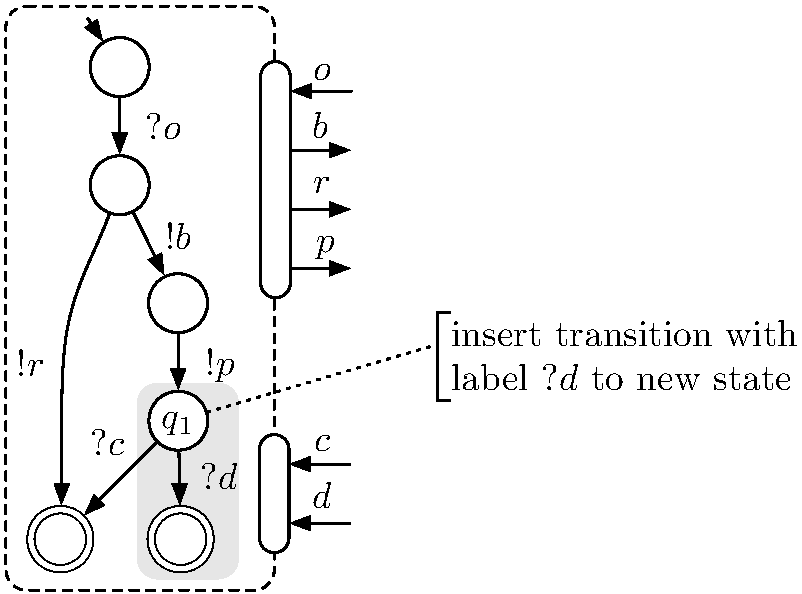
\includegraphics[scale=0.45]{correction/fixedsa}
\caption{Matching-based edit distance applied to the customer's service.}
\label{fig:fixedsa}
\end{figure}
%%%%%%%%%%%%%%%%%%%%%%%%%%%%%%%%%%%%%%%%%%%%%%%%%%%%%%%%%%%%%%%%%%%%%%%%%%%%%%

\Autoref{fig:fixedsa} shows the result of the application of the matching-based edit distance to the service automaton of \autoref{fig:corsa} assuming a discount factor $p=0.7$ and a label similarity function $L$, which assigns $1.0$ to equal labels and $0.5$ to any other label pair. The states are annotated with edit actions. Interestingly, the values of $p$ and $L$ had little impact on the correction of the example. Only for extreme values (\eg, $p=1.0$ or $L(x,x)=1.0$ for all labels $x$), the result changed. The traveler service automaton was automatically generated from a \acronym{WS-BPEL} process and the state in which a modification has to be made can be mapped back to the original \acronym{WS-BPEL} activity. In the example, a \bpel{receive} activity has to be replaced by a \bpel{pick} activity with an additional \bpel{onMessage} branch to receive the decline message. The result would then coincide with the desired result of \autoref{fig:fix2}.





%%%%%%%%%%%%%%%%%%%%%%%%%%%%%%%%%%%%%%%%%%%%%%%%%%%%%%%%%%%%%%%%%%%%%%%%%%%%%%%
\section{Experimental results}\label{sect:experimental}
%%%%%%%%%%%%%%%%%%%%%%%%%%%%%%%%%%%%%%%%%%%%%%%%%%%%%%%%%%%%%%%%%%%%%%%%%%%%%%%

The original simulation algorithm of~\cite{SokolskyKL_2006_tacas} to calculate a weighted quantitative simulation between two service automata $A_{1}$ and $A_{2}$ (cf.~\autoref{def:wwqs}) needs to check at most $|Q_{A_{1}}|\cdot |Q_{A_{2}}|$ state pairs. The extension to calculate the matching between a service automaton $A$ and an operating guideline~$B^\varphi$ (cf.~\autoref{def:wqmatching}) takes the operating guideline's formulae and the resulting label permutations into consideration. The length of the operating guideline's formulae is limited by the maximal degree of the nodes which again is limited by the number of open message channels, because operating guidelines are by definition $\tau$-free and  deterministic. Let~$\M^\open$ be the set of open message channels of $B^\varphi$. Then, for each state pair, at most $2^{|\M^\open|}$ satisfying assignments have to be considered. The number of permutations is again limited by the maximal node degree such that at most $|\M^\open|!$ permutations have to be considered for each state pair and assignment. This results in at most $|Q_{A}|\cdot |Q_{B}| \cdot 2^{|\M^\open|} \cdot |\M^\open|!$ comparisons.

Although the extension toward a formula-checking edit distance has a discouraging worst-case complexity, operating guidelines of real-life services tend to have simple formulae, a relatively small interface compared to the number of states, and a low node degree. As a proof of concept, we implemented the edit distance in a software prototype Rachel~\cite{rachel}. It takes an acyclic deterministic service automaton and an acyclic operating guideline as input and calculates the edit actions necessary to achieve a matching with the operating guideline. We evaluated the prototype again using service automata generated for \acronym{WS-BPEL} services. In this experiment, we restricted ourselves to acyclic services and translated only the positive control flow (\ie, no exceptional behavior). The edit distance usually could be calculated within few seconds. The prototype exploits that a lot of subproblems overlap and uses dynamic programming techniques~\cite{Bellman_1957} to cache and reuse intermediate results which significantly accelerates the runtime. For the examples of the experiment, we observed a cache hit ratio of about 97\,\%. However, no example used more than 5 \acronym{MB} of memory. The experiments were conducted using a computer with a 3~\acronym{GH}z processor. \Autoref{tab:exp} summarizes the results.

%%%%%%%%%%%%%%%%%%%%%%%%%%%%%%%%%%%%%%%%%%%%%%%%%%%%%%%%%%%%%%%%%%%%%%%%%%%%%%
\begin{table}
\caption{Experimental results on service correction using Rachel.}
\centering\footnotesize
\begin{tabular*}{\textwidth}{@{\extracolsep{\fill}}lcccrlr}
\toprule
service & $|\E_{\mathcal{P}}|$ & $|Q_{A}|$ (SA) & $|Q_{B}|$ (OG) & \multicolumn{2}{c}{search space} & time (sec) \\  \midrule
Online Shop		& $16$ & $222$ & $153$ && $10^{2033}$ & $2$ \\ %&& 238616 & 195783 & 4 \\ % DKE 3
Supply Order		& $7$  &   $7$ &  $96$ && $10^{733}$ & $1$ \\ %&& 19056 & 114 & 1 \\ %MEGA Bestellung Hauslieferung
Customer Service	& $9$  & $104$ &  $59$ && $10^{108}$ & $2$ \\ %&& 114702 & 1000 & 3 \\ %MEGA
Internal Order	& $9$ &  $14$ & $512$ & $\quad>\hspace{-0.8em}$&$10^{4932}$ & $100$ \\ % 101508518 & 227473 & 602 & 211 \\ %MEGA (Normale Bestellung)
Credit Preparation&  $5$ &  $63$ &  $32$ && $10^{36}$ & $1$ \\ %101508522 & 68191 & 489 & 2 \\ %MEGA
Register Request	&  $6$ &  $19$ &  $24$ && $10^{25}$ & $0$ \\ %1393722303 & 4086 & 85 & 0\\ %Gedilan (Melderegister)
Car Rental		&  $7$ &  $50$ &  $50$ && $10^{144}$ & $3$ \\ \midrule[0.1ex] %& 165430 & 492 & 6 \\ %MEGA (Car Return)
Order Process	& $8$  &  $27$ &  $44$ && $10^{222}$ & $0$ \\ % && 4796 & 133 & 0 \\ %\acronym{BPEL}-Spec
Auction Service	& $6$	 &  $13$ & $395$ && $10^{12}$ & $0$ \\ %&& 395 & 33 & 0 \\ %\acronym{BPEL}-Spec
Loan	 Approval	& $6$  &  $15$ &  $20$ && $10^{17}$ & $0$ \\ %&& 758 & 50 & 0 \\ %\acronym{BPEL}-Spec
Purchase Order	& $10$ & $137$ & $168$ & $>\hspace{-0.8em}$&$10^{4932}$ & $193$ \\ %&& 5754625 & 3341 & 391\\ %\acronym{BPEL}-Spec
\bottomrule
\end{tabular*}
\label{tab:exp}
\end{table}
%%%%%%%%%%%%%%%%%%%%%%%%%%%%%%%%%%%%%%%%%%%%%%%%%%%%%%%%%%%%%%%%%%%%%%%%%%%%%%

As we had no access to real-life service compositions, we could only evaluate our approach in the case of service compositions consisting of two services. The first seven services of \autoref{tab:exp} are \acronym{WS-BPEL} processes of a consulting company; the last four services were taken from the \acronym{WS-BPEL} specification~\cite{standard_bpel}. The services were first translated into service automata using the compiler \bpelowfn~\cite{Lohmann_2007_hubtr212}. For these service automata, the operating guidelines were calculated using the tool Wendy~\cite{LohmannW_2009_wendy}. Note that the complexity of the calculation of the edit distance is independent of the fact whether the service automaton matches the operating guideline or not. In case no partner service was available, we synthesized a strategy with Wendy and manually added a few mistakes that lead to incompatibility. As we can see from \autoref{tab:exp}, the services' interfaces are rather small compared to their number of states.

Column ``search space'' of \autoref{tab:exp} lists the number of acyclic deterministic services characterized by the operating guideline. This number is calculated by Rachel and is bounded by $10^{4932}$ due to technical reasons\,---\,this is the maximal number that can be represented by an 80 bit floating point data type. All these services are correct partner services and have to be considered during the search for the most similar service. The presented algorithm exploits the compact representation of the operating guideline and allows to efficiently find the most similar service from more than $10^{2000}$ candidates.

For most services, the calculation only takes a few seconds. The ``Internal Order'' and ``Purchase Order'' services are exceptions. The operating guidelines of these services have long formulae with a large number of satisfying assignments (about ten times larger than those of the other services) yielding a significantly larger search space. Notwithstanding the larger calculation time, the service fixed by the calculated edit actions is correct by design, and the calculation time is surely an improvement compared to iterative manual correction.

\Autoref{fig:correction:rachel} depicts the output of the tool Rachel. It consists of a graphical representation of the incorrect service automaton whose edges are annotated with edit actions. Different colors (green for insertion, yellow for modification, and red for removal) symbolize the respective edit actions. The proposed edit actions are additionally given as textual output.

%%%%%%%%%%%%%%%%%%%%%%%%%%%%%%%%%%%%%%%%%%%%%%%%%%%%%%%%%%%%%%%%%%%%%%%%%%%%%%
\begin{figure}
\centering
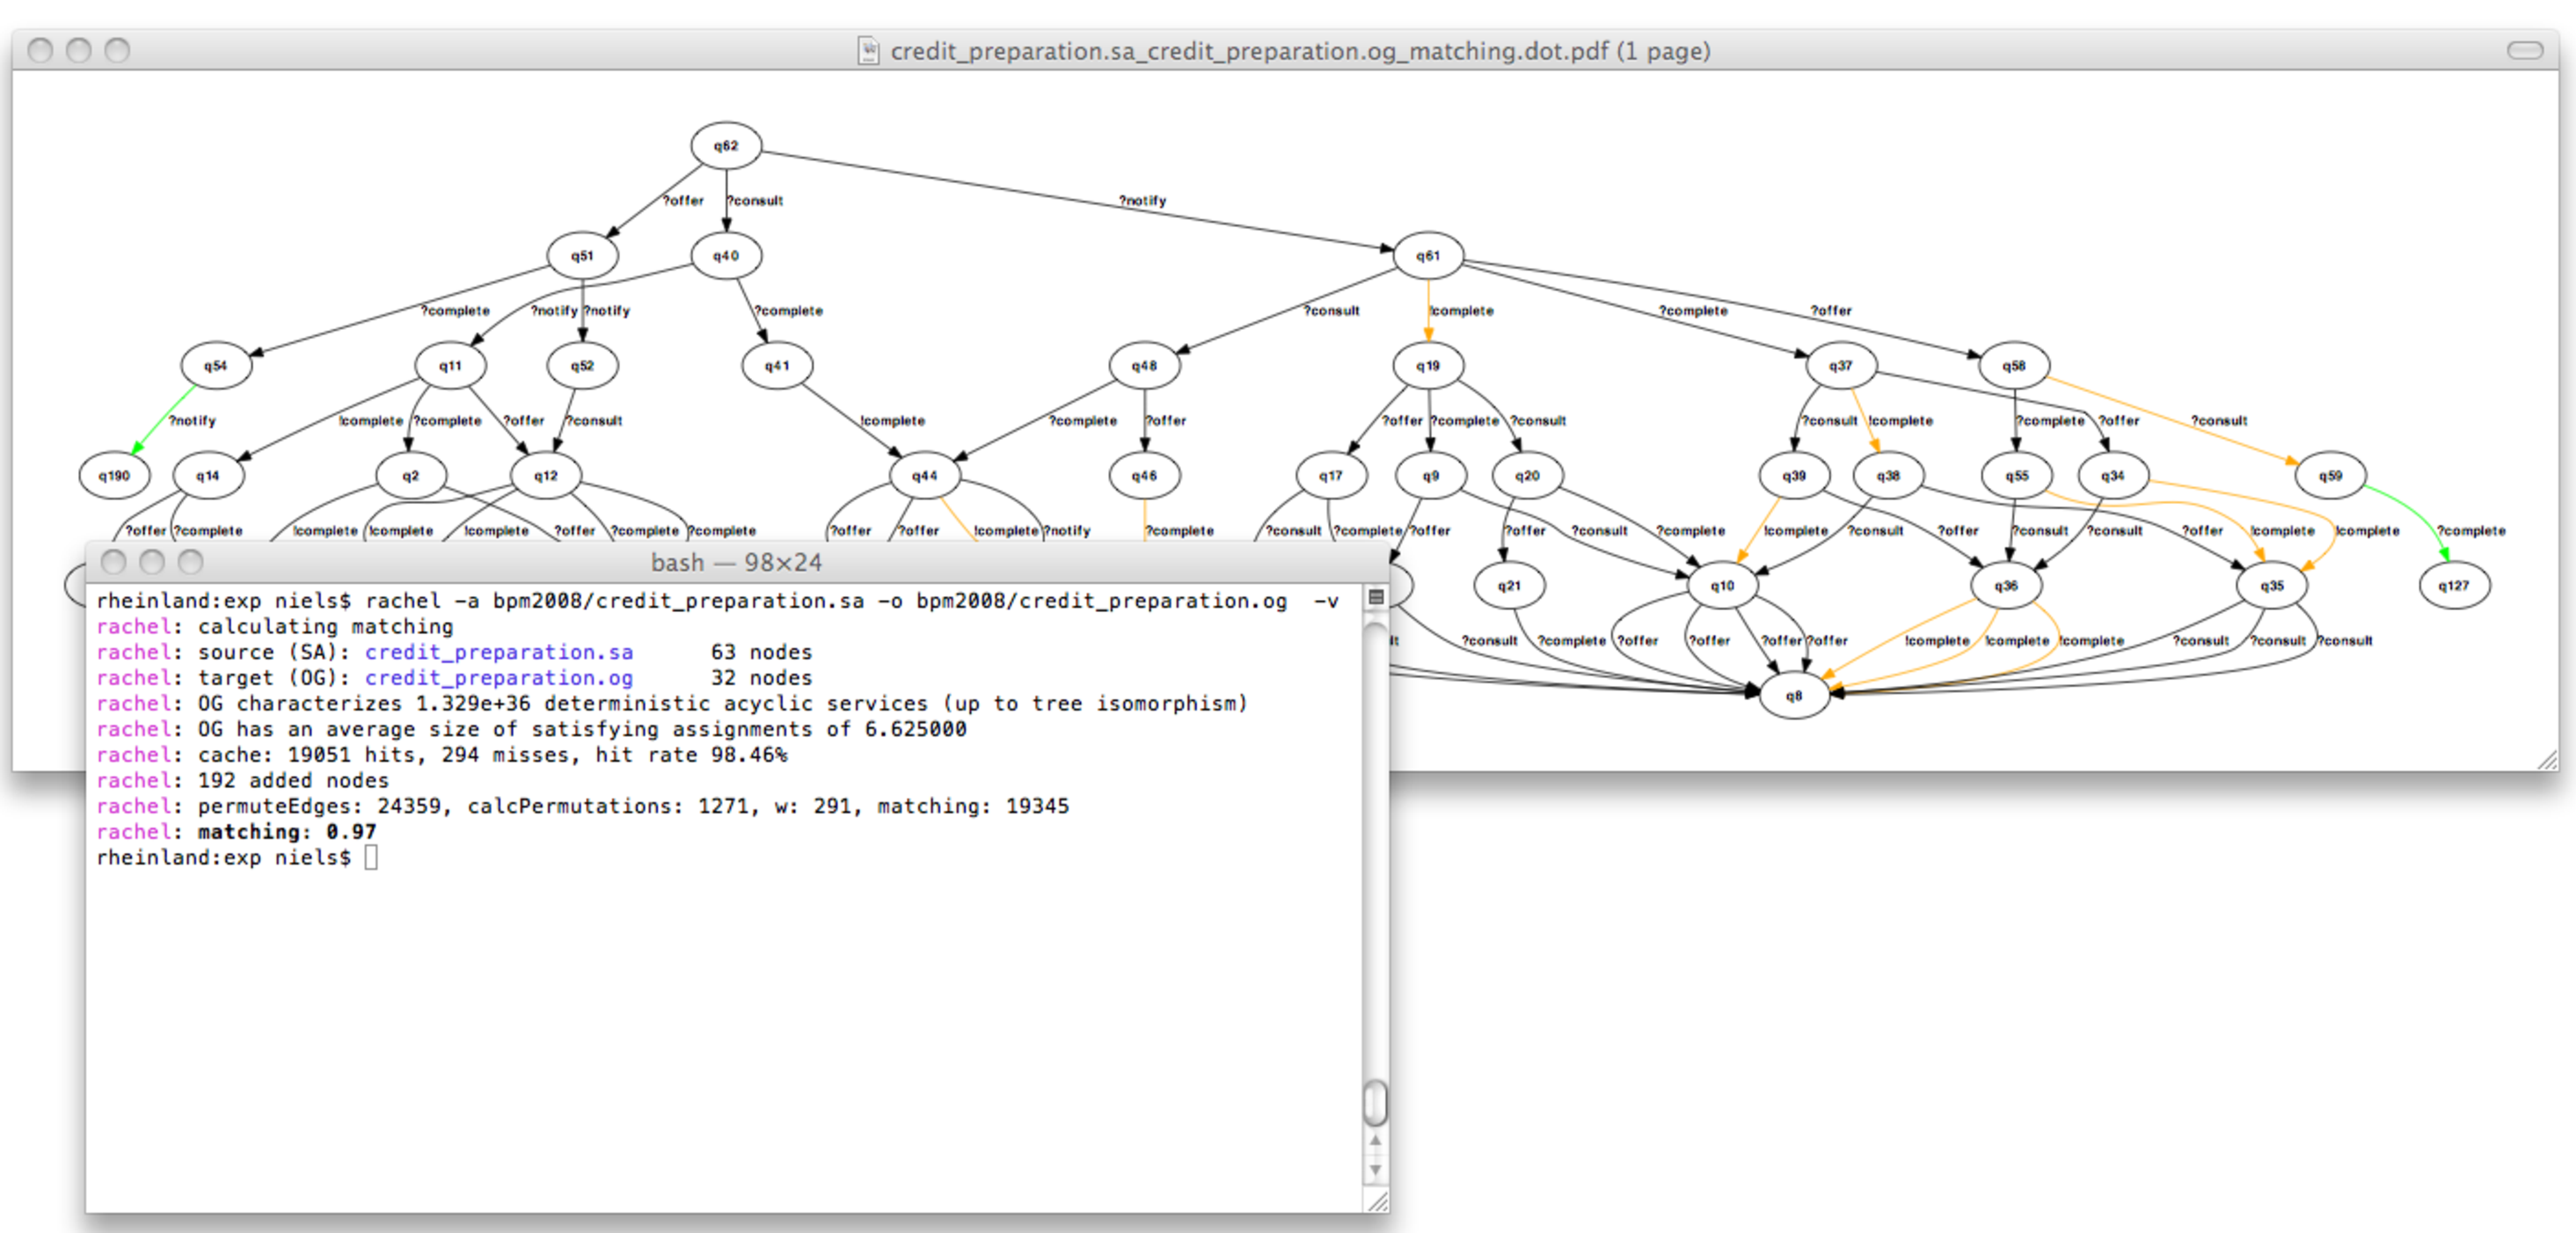
\includegraphics[width=\textwidth]{correction/rachel}
\caption{Correction output of the tool Rachel for the credit preparation example.}
\label{fig:correction:rachel}
\end{figure}
%%%%%%%%%%%%%%%%%%%%%%%%%%%%%%%%%%%%%%%%%%%%%%%%%%%%%%%%%%%%%%%%%%%%%%%%%%%%%%





%%%%%%%%%%%%%%%%%%%%%%%%%%%%%%%%%%%%%%%%%%%%%%%%%%%%%%%%%%%%%%%%%%%%%%%%%%%%%%%
\section{Related work}\label{sect:related}
%%%%%%%%%%%%%%%%%%%%%%%%%%%%%%%%%%%%%%%%%%%%%%%%%%%%%%%%%%%%%%%%%%%%%%%%%%%%%%%

The presented matching edit distance is related to several aspects of current research in many areas of computer science:


\paragraph{Automated debugging.}

In the field of model checking, the explanation of errors by using distance metrics~\cite{GroceCKS_2006_sttt} has received much attention. Compared to the approach presented in this paper, these works focus on the explanation and location of single errors in classical~C (\ie, low-level) programs. The derived information is used to support the debugging of an erroneous program.


\paragraph{Service matching.}

Many approaches exist to discover a similar partner service. \citet{CorralesGB_2006_otm} and \citet{GrigoriCB_2008_is} investigate the matching of \acronym{WS-BPEL} processes and Web service conversations, respectively. Both approaches rely on graph isomorphisms and do not consider service behavior. \citet{DijkmanDG_2009_bpm} compare several heuristic approaches to speed up matching between business processes and report promising runtimes even for larger sets of processes. Compared to our approach, they focus only on the structure of a process rather than on its behavior. Other approaches~\cite{WuW_2005_scc,BianchiniAM_2006_emoi} use ontologies and take the semantics of activities into account, but do not focus much on the behavior or message exchange. \citet{GunayY_2007_ecweb} represent the behavior of a service as a language of traces and apply string edit distances to compare services. This approach, however, cannot be used in the setting of asynchronously communicating services where the moment of branching is crucial to avoid deadlocks.


\paragraph{Service similarity and versioning.}

The change management of business processes and services is subject of many recent works. An overview of what can differ between otherwise similar services is given by \citet{Dijkman_2007_edoc,Dijkman_2008_bpm}. The reported differences go beyond the behavioral level and take authorization aspects under consideration. \citet{WeberRR_2007_caise} give an overview of frequent change patterns occurring in the evolution of a business process model. Beside the already mentioned basic operations (adding, changing, and removing of edges or nodes), complex operations such as extracting    subprocesses are presented. With a \emph{version preserving graph}, a technique to represent different versions of a process model is introduced by~\citet{ZhaoL_2007_bpm}. This technique was made independent of a change log by~\citet{KuesterGFE_2008_bpm}. Again, versioning relies on the structure of the model rather than on its behavior. \citet{Ait-BachirDF_2008_icsoc} investigate behavioral differences in terms of simulation.  They compare behavioral incompatibilities between two services and elaborate an edit distance to overcome these incompatibilities. Their result is much related to our simulation-based edit distance, but only consider synchronous communication.

\citet{LiRW_2009_bpm} apply an edit distance to find, given several process variants, a reference process model which is most similar to all variants with respect to structural change operations. This approach could be applied to our correction setting by treating each strategy that is characterized by an operating guideline as variant model and the most similar correct participant as a reference model. However, experimental results are only reported for up to 100 processes.


\paragraph{Service mediation.}

An alternative to changing a service to a\-chieve compatibility in a choreography offer \emph{service mediators} (sometimes called adapters)~\cite{BrogiP_2006_icsoc,DumasSW_2006_bpm,GierdsMW_2010_tcs}. Service mediation is rather suited to fit existing services, whereas our approach aims at supporting the design and modeling phase of a service choreography. Still, a mediator between the customer service on the one hand and the travel agency and the airline service on the other hand (cf.~\autoref{fig:chor}) would have to receive the airline's decline message and create a confirmation message for the customer which is surely unintended. Furthermore, several service mediation approaches assume total perception of the participants' internal states during runtime~\cite{NezhadBMCC_2007_www}.

\medskip

The difference between all mentioned related approaches and the setting of this paper is that these approaches either focus on low-level programs or mainly aim at finding \emph{structural} (and certainly not simulation-based) differences between \emph{two} given services and are therefore not applicable to find the most similar service from a large set (cf.~\autoref{tab:exp}) of candidates. 





%%%%%%%%%%%%%%%%%%%%%%%%%%%%%%%%%%%%%%%%%%%%%%%%%%%%%%%%%%%%%%%%%%%%%%%%%%%%%%%
\section{Conclusion and Future Work}\label{sect:conclusion}
%%%%%%%%%%%%%%%%%%%%%%%%%%%%%%%%%%%%%%%%%%%%%%%%%%%%%%%%%%%%%%%%%%%%%%%%%%%%%%%

We presented an edit distance to compute the edit actions necessary to correct a faulty service to interact in a choreography in a compatible manner. We defined this edit distance in two steps. First, we defined an edit distance based on existing work on a quantitative similarity measure, which was originally defined to compare behavior with respect to a simulation relation. Second, we adjusted this approach to suite our setting of comparing a service automaton with a set of service automata, implicitly characterized as operating guideline. The edit distance (\ie, the actions needed to correct the service) can be automatically calculated using a prototypic implementation. Together with translations from~\cite{Lohmann_2007_wsfm} and to~\cite{LohmannK_2008_mod} \acronym{WS-BPEL} processes and the calculation of the characterization of all correct partner services (the operating guideline)~\cite{LohmannMSW_2006_bpm,LohmannMW_2007_atpn}, an integrated tool chain to analyze and correct \acronym{WS-BPEL}-based choreographies is available. As the edit distance itself is based on service automata, it can be easily adapted to other modeling languages such as \acronym{UML} activity diagrams~\cite{standard_uml} or \acronym{BPMN}~\cite{standard_bpmn} using Petri net or automaton-based formalizations.

The edit distance is an important tool to support the development of correct service compositions. With its help, we are not just able to detect and diagnose incompatibilities, but also to \emph{propose} corrections. The corrected services try to reuse as much behavior of the original faulty service, yet is still guaranteed to be \emph{correct by design}. Although the approach presented in this chapter is still in its infancy and is subject to many restrictions (the structure must be acyclic and deterministic, and final states must be sink states), it is likely to be applicable in several application scenarios. For instance, \citet{ParnjaiSW_2009_zeus} use the presented edit distance to correct a service $A$ such that it can substitute another service $B$; that is, the corrected service must not exclude strategies of $B$. Another application could be the organization of services in a service registry (cf.~\autoref{fig:soatriangle}): This registry could be partitioned using the similarity of services with respect to certain typical ``key services''. This partition then could narrow down the search space for a provider service by only searching in these partitions that are sufficiently similar to the query service. Likewise, the edit distance can be used to rank results as reported by~\citet{DijkmanDG_2009_bpm}.

\medskip

However, several questions still remain open. First, the choice \emph{which} service causes the incompatibility and hence needs to be fixed is not always obvious and needs further investigation. For instance, the choreography in \autoref{fig:chor} could also have been corrected by adjusting the airline service. Even worse, the composition depicted in \autoref{fig:corr:counter} shows that for some compositions, the behavior of more than one service needs to be corrected.

A further aspect to be considered in future research is the choice of the \emph{cost function} used in the algorithm, because it is possible to set different values for any transition pairs. This could be, for instance, achieved with questionnaires such as reported by \citet{Wombacher_2006_otm}. Semantic information on message contents (\eg, derived from an ontology) and relationships between messages can be incorporated to refine the correction. For example, the insertion of the receipt of a confirmation message can be penalized less than the insertion of sending an additional payment message.

The similarity function could also be adjusted by taking the \emph{execution frequencies} of activities into account: \citet{MedeirosAW_2008_dke} present a novel process mining algorithm that not only considers execution traces, but also distinguished frequently executed activities (``highways'') from rarely used activities (``dirt roads''). They report how this information can be used to improve the quality of mined process models.

Another important field of research is to further increase the performance of the implementation by an early omission of suboptimal edit actions. For instance, heuristic guidance metrics such as used in the $\mbox{A}\!^\ast$~algorithm~\cite{HartNR_1968_ssc} may greatly improve runtime performance.

Finally, a translation of the matching edit distance of \autoref{def:wqmatching} into a linear optimization problem~\cite{Schrijver_1998} may also help to cope with cyclic and nondeterministic services.
